%----------------------------------------------------------------------------------------
%	PACKAGES AND THEMES
%----------------------------------------------------------------------------------------
\PassOptionsToPackage{table}{xcolor}
\documentclass[aspectratio=169,xcolor=dvipsnames,svgnames,x11names,fleqn]{beamer}
% \documentclass[aspectratio=169,xcolor=dvipsnames,fleqn]{beamer}

\usetheme{RedVelvet}

\usefonttheme[onlymath]{serif}



\usepackage{xspace}
\usepackage{amsmath}
\usepackage{amssymb}
\usepackage{amsfonts}
\usepackage{color}
\usepackage{physics}
% \usepackage{mathbb}
\usepackage{rahul_math}
\usepackage{bigints}
\usepackage{hyperref}

\usepackage{graphicx} % Allows including images
\usepackage{booktabs} % Allows the use of \toprule, \midrule and \bottomrule in tables
\usepackage{tikz,pgfplots}
\usepackage{subfigure}
\usetikzlibrary{arrows}
\usepackage{minted}
\definecolor{LightGray}{gray}{0.9}
\definecolor{cream}{rgb}{0.92, 0.9, 0.55}
\definecolor{lightblue}{rgb}{0.68, 0.85, 0.9}


\usepackage{xcolor-material}
\usetikzlibrary{fit}
\tikzset{%
apple/.pic={
  \fill [MaterialBrown] (-1/8,0)  arc (180:120:1 and 3/2) coordinate [pos=3/5] (@)-- ++(1/6,-1/7)  arc (120:180:5/4 and 3/2) -- cycle;
  \fill [MaterialLightGreen500] (0,-9/10)  .. controls ++(180:1/8) and ++(  0:1/4) .. (-1/3,  -1) .. controls ++(180:1/3) and ++(270:1/2) .. (  -1,   0) .. controls ++( 90:1/3) and ++(180:1/3) .. (-1/2, 3/4) .. controls ++(  0:1/8) and ++(135:1/8) .. (   0, 4/7)
}
}

\newcommand{\leftdoublequote}{\textcolor{blue}{\scalebox{3}{``}}}

\newcommand{\rightdoublequote}{\textcolor{blue}{\scalebox{3}{''}}}


\usepackage{textcomp}
\usepackage{fontawesome}

\usepackage{overpic}

%----------------------------------------------------------------------------------------
%	TITLE PAGE
%----------------------------------------------------------------------------------------

\usepackage{tikz-qtree,tikz-qtree-compat}
\usetikzlibrary{calc}


\title[CPE 486/586: Machine Learning]{CPE 486/586: Machine Learning for Engineers} % The short title appears at the bottom of every slide, the full title is only on the title page
\subtitle{01 Introduction}

\author[Rahul Bhadani] {{\Large \textbf{Rahul Bhadani}}}

\institute[UAH] % Your institution as it will appear on the bottom of every slide, maybe shorthand to save space
{
    Electrical \& Computer Engineering,  The University of Alabama in Huntsville
}
\date

% \titlegraphic{
%    \includegraphics[width=0.4\linewidth]{figures/UAH_primary.png}
% }

\begin{document}

%-------------------------------------------------
\begin{frame}
  \titlepage
\end{frame}

%-------------------------------------------------
\begin{frame}{Outline}
  \backgroundtableofcontents
\end{frame}

%%%%%%%%%%%%%%%%%%%%%%%%%%%%%%%%%%%%%%%%%%%%%%%%%%%%%
\section{Course Logistics}

%-----------------------------------------.-------
\begin{frame}{About Me}
    \begin{columns}[c] % The "c" option specifies centered vertical alignment while the "t" option is used for top vertical alignment

        \column{.60\textwidth} % Left column and width
        \textbf{Rahul Bhadani} \\
        Assistant Professor \\
        Electrical and Computer Engineering \\
        The University of Alabama in Huntsville \\
        Office: 217-H \\
        Email: {\color{MediumRed}{rahul.bhadani@uah.edu}} \\
        Web: {\color{MediumRed}\url{https://rahulbhadani.github.io/}}

        \column{.30\textwidth} % Right column and width
        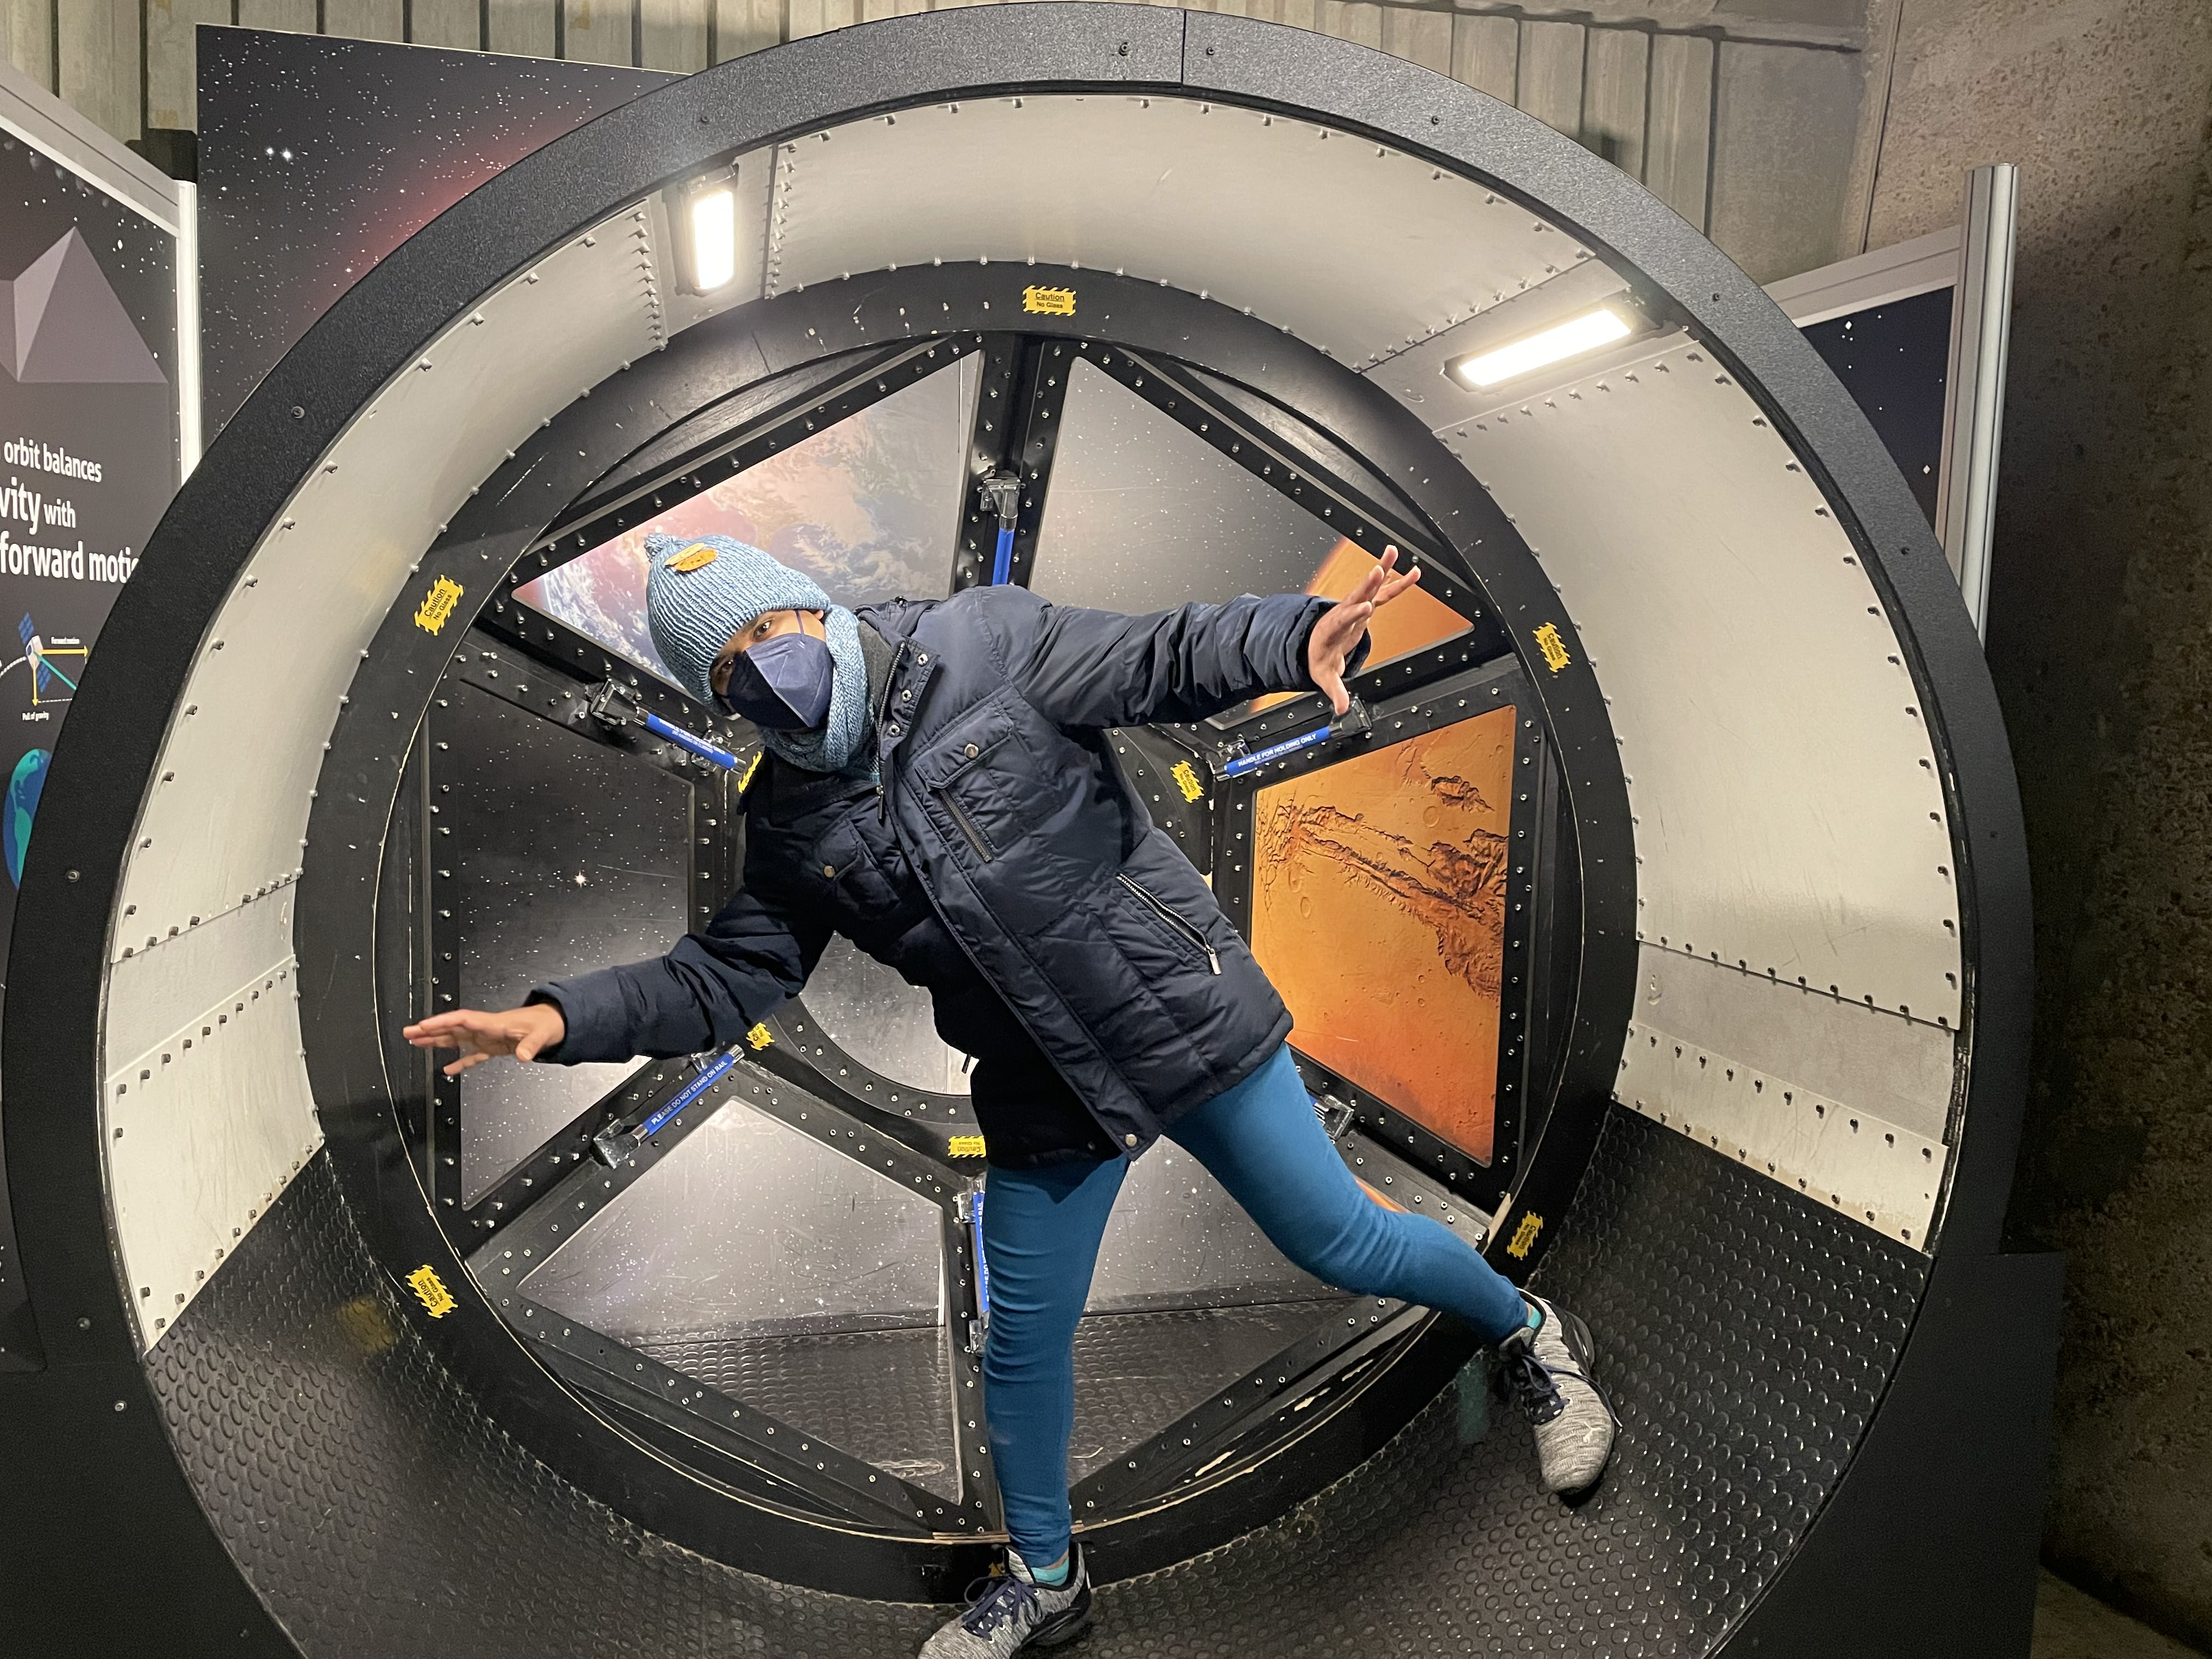
\includegraphics[width=.89\textwidth]{figures/intro_rkb.jpg}
    \end{columns}
    
    \begin{block}{Research Interests}
    Cyber-physical Systems,
    Intelligent Transportation, 
    Connected-and-Autonomous Driving, 
    Applied machine learning,
    Quantum Information Science
    \end{block}
\end{frame}


%-------------------------------------------------

\begin{frame}{Course Logistics
}
  \begin{columns}[T] % align columns at the top
    \begin{column}{0.5\textwidth}
      \textbf{Lecture:} \\
      M/W 4:20 PM - 5:40 PM \\
      \vspace{0.3cm}
      \textbf{Location:} \\
      ENG 239 \\
      
    \end{column}
    \begin{column}{0.5\textwidth}
      \textbf{Office Hours:}
      \begin{itemize}
        \item TBD
      \end{itemize}
      \textbf{Instructor Email:} rahul.bhadani@uah.edu
    \end{column}
  \end{columns}
\end{frame}

%-----------------------------------------
\begin{frame}{Textbooks}

\end{frame}

%-----------------------------------------
\begin{frame}{Grading}

\footnotesize

\begin{columns}
    \column{0.6\linewidth}

\begin{center}

\textbf{CPE 486}

\begin{tabular}{lp{1in} l l l}
\textbf{Homework:} & 30\% \\
 \textbf{Quizzes:} &  5\%\\
\textbf{Attendance/In-Class Participation:} & 5\%\\
\textbf{Mid-term Exam 1:} & 15\%  \\
\textbf{Mid-term Exam 2:} & 15\%  \\
\textbf{Final Exam:} & 30\%  \\
\end{tabular}

\textbf{CPE 586}

\begin{tabular}{lp{1in} l l l}
\textbf{Homework:} & 25\% \\
 \textbf{Quizzes:} &  5\%\\
\textbf{Attendance/In-Class Participation:} & 5\%\\
\textbf{Mid-term Exam 1:} & 15\%  \\
\textbf{Mid-term Exam 2:} & 15\%  \\
\textbf{Final Exam:} & 30\%  \\
\textbf{Project Report:} & 5\%  \\

\end{tabular}

\end{center}
\column{0.4\linewidth}
\begin{tabular}{|p{3cm}|p{1.5cm}|}
\hline
\multicolumn{2}{|c|}{\textbf{Grading Scale}} \\ \hline
\textbf{Percentage} & \textbf{Grade} \\ \hline
90\% - 100\% & A \\ \hline
75\% - 89\% & B \\ \hline
60\% - 74\% & C \\ \hline
45\% - 59\% & D \\ \hline
0\% - 44\% & F \\ \hline
\end{tabular}
\end{columns}
\end{frame}


\begin{frame}{Homework Policy}
\begin{itemize}
\item Each late submission will be penalized by 10\% per day for up to 5 days maximum, thereafter, if later, one will receive 0 credit. 
\item Solution to homework will be posted 5 days after the due date.
\end{itemize}

\end{frame}

\begin{frame}{Classwork}

\begin{itemize}
\item Each lecture will be followed by in-class problem-solving that students will turn in the next lecture day. If you miss the lecture day (either the day it is handed to you, or the day you need to turn in), you will not receive any credit.

\item There will be intermediate small tests to assess your skills based on lectures and the classwork. This portion will count towards your classwork credits.
\end{itemize}



\end{frame}

\begin{frame}{Attendance Policy}

\begin{itemize}
\item Must attend all lectures.
\item Two unexcused absences permitted.
\item No option to make up for classwork.
\end{itemize}

\end{frame}

%-----------------------------------------
\begin{frame}{Exam Schedule}
\begin{tabular}{|p{3cm}|p{5cm}|p{5cm}|}
\hline
\multicolumn{3}{|c|}{\textbf{Exam Dates}} \\ \hline
\textbf{Exam} & \textbf{Date} & \textbf{Time} \\ \hline
Mid-Term 1 & Wednesday, September 24, 2025 & 4:20 PM to 5:40 PM\\ \hline
Mid-Term 2 & Wednesday, November 5, 2025 & 4:20 PM to 5:40 PM\\ \hline
Final Exam & Friday, December 12, 2025 & 3:00 PM to 5:30 PM\\ \hline
\end{tabular}
\end{frame}

%-----------------------------------------
\begin{frame}{Tentatative Topics}
\tiny
\begin{itemize}
	\item \color{DarkRed} \underline{Course Introduction, Mathematical Preliminaries}: Linear Algebra, Probability and Statistics
	

		\item \color{DarkRed} \underline{Tools for Machine Learning}: Installing Python, Unix Terminal, SSH, Git, Jupyter Notebook, Markdown, Latex, Package Manager, 
	
	
 
    \item \color{DarkRed} \underline{Scientific Python} Numpy, Scikit-learn, IPython \& Jupyter Notebook, Matplotlib, Pandas, Matrix Algebra with Python,  Root-finding using Newton Raphson Method, Probability and Statistics with Python, PyTorch for Linear Algebra

% https://www.youtube.com/watch?v=geFER2oVvvU
    \item  \color{DarkRed} \underline{Optimization and Gradient Descent} Continuous Optimization, Optimization Using Gradient Descent,  Univariate Optimization, Multivariate Optimization, Constrained Optimization and Lagrange Multipliers, Convex Optimization, Methods of Least Square, Implementation in Pandas, Scipy and Pytorch
    
    \item   \color{DarkRed} \underline{Supervised Learning -- Regression}  Simple Linear Regression, Variance Estimation, Goodness of Fit, Confidence-band, Matrix approach to Regression, Multiple Linear Regression, Polynomial Regression, Locally Weighted Regression, Kernel Methods for Regression, Implementation in Scipy and PyTorch
    
    \item  \color{DarkRed} \underline{Supervised Learning -- Logistics Regression} Classification Problem, Logistics Function, Model Assessment

    \item  \color{DarkRed} \underline{Overfitting and Regularization} Overfitting, Underfitting, Bias-Variance Tradeoff, Regularization, Ridge-Regression, LASSO, Elastic-Net
    
    \item \color{DarkRed} \underline{Dimensionality Reduction and Feature Selections}  Maximum Variance Perspective, Projection Perspective, Eigenvector Computation and Low-Rank Approximations, Principal Component Analysis, Latent Variable Perspective,  Feature Selection, Data Transforms, Implementation using Scikit-learn, Pandas, and Pytorch
    
    \item   \color{DarkRed}  \underline{Supervised Learning -- Support Vector Machine (SVM)} Linear Classifier, Concept of Hyperplane, Hard Margin SVM, Soft-Margin SVM, Kernel-based SVM, Implementation using Scipy
      
   

     \item  \color{DarkRed} \underline{Unsupervised Learning -- Classification} Clustering techniques, K-means, Hierarchical Clustering, Agglomerative Clustering, DBSCAN, Graph-based Clustering, Expectation Maximization Algorithms, Gaussian Mixture Model, Evaluating Cluster Qualities, Implementation using Scipy

      \item  \color{DarkRed} \underline{Introducing Deep Learning -- Neural Networks} Perceptron, Multi-layer Perceptron, Nonlinear Activation Functions, Backpropagation Algorithms, Vectorization and Batch Techniques, Neural Network Layers, Training Neural Networks, Learning Rates and Optimization Techniques in Neural Network, Implementation using PyTorch
    
   
\end{itemize}
\end{frame}

\begin{frame}{Getting ML Specific Help with Python}
Where can I get resources to help with Python programming?
\begin{itemize}
%    \item Many of the figures that appear in the slides were written with Python ({\color{MediumRed}\url{https://github.com/gditzler/ML-Lecture-Figures}})
    \item Python for Everybody by Dr. Charles Severance ({\color{MediumRed}\url{https://www.youtube.com/watch?v=PKrC027wIUU&list=PLAtoCfxWRIErTozMKGdHmUieMuQDGEoEJ}}) is a great place to refresh your Python
    \item Sklearn has some extremely helpful documentation pages ({\color{MediumRed}\url{https://scikit-learn.org/stable/index.html}})
    \item Matplotlib: the most used visualization tool in Python: ({\color{MediumRed}\url{https://matplotlib.org/stable/tutorials/index.html}})

	\item Polars for Data Analysis: {\color{MediumRed}\url{https://docs.pola.rs/user-guide/getting-started/}}

    \item Learning PyTorch with Examples: 
    ({\color{MediumRed}\url{https://pytorch.org/tutorials/beginner/pytorch_with_examples.html}})
\end{itemize} 


\end{frame}

%------------------------------------------------
\begin{frame}{How to get help for this course?}
\begin{itemize}
    \item Ask questions in the class without hesitation. No question is silly.
    \item Utilize office hours to the maximum extent.
    \item Start your homework as soon as it is posted. The more you delay, the chance of your success will diminish.
    \item Do additional self-reading related to topics covered in the class.
\end{itemize}

\begin{texample}
Remember, you are here to learn the material in this course, and not just pass it.
\end{texample}
\end{frame}

%-----------------------------------------
\begin{frame}{In-Class Activity}
  \centering
  \textbf{Introduce Yourself} \\[1em]
  
  \begin{block}{}
    \begin{itemize}
      \item Why do you want to take this course?
      \item What are your research intersts? How are you planning to utilize Machine Learning in your research/career?
    \end{itemize}
  \end{block}

\end{frame}

%%%%%%%%%%%%%%%%%%%%%%%%%%%%%%%%%%%%%%%%%%%%%%%%%%%%%
%%%%%%%%%%%%%%%%%%%%%%%%%%%%%%%%%%%%%%%%%%%%%%%%%%%%%
\begin{sectionframe}{\faRocket}{Introduction to the Course}
\end{sectionframe}


%------------------------------------------------
\begin{frame}{Contributors to ML}
\begin{center}
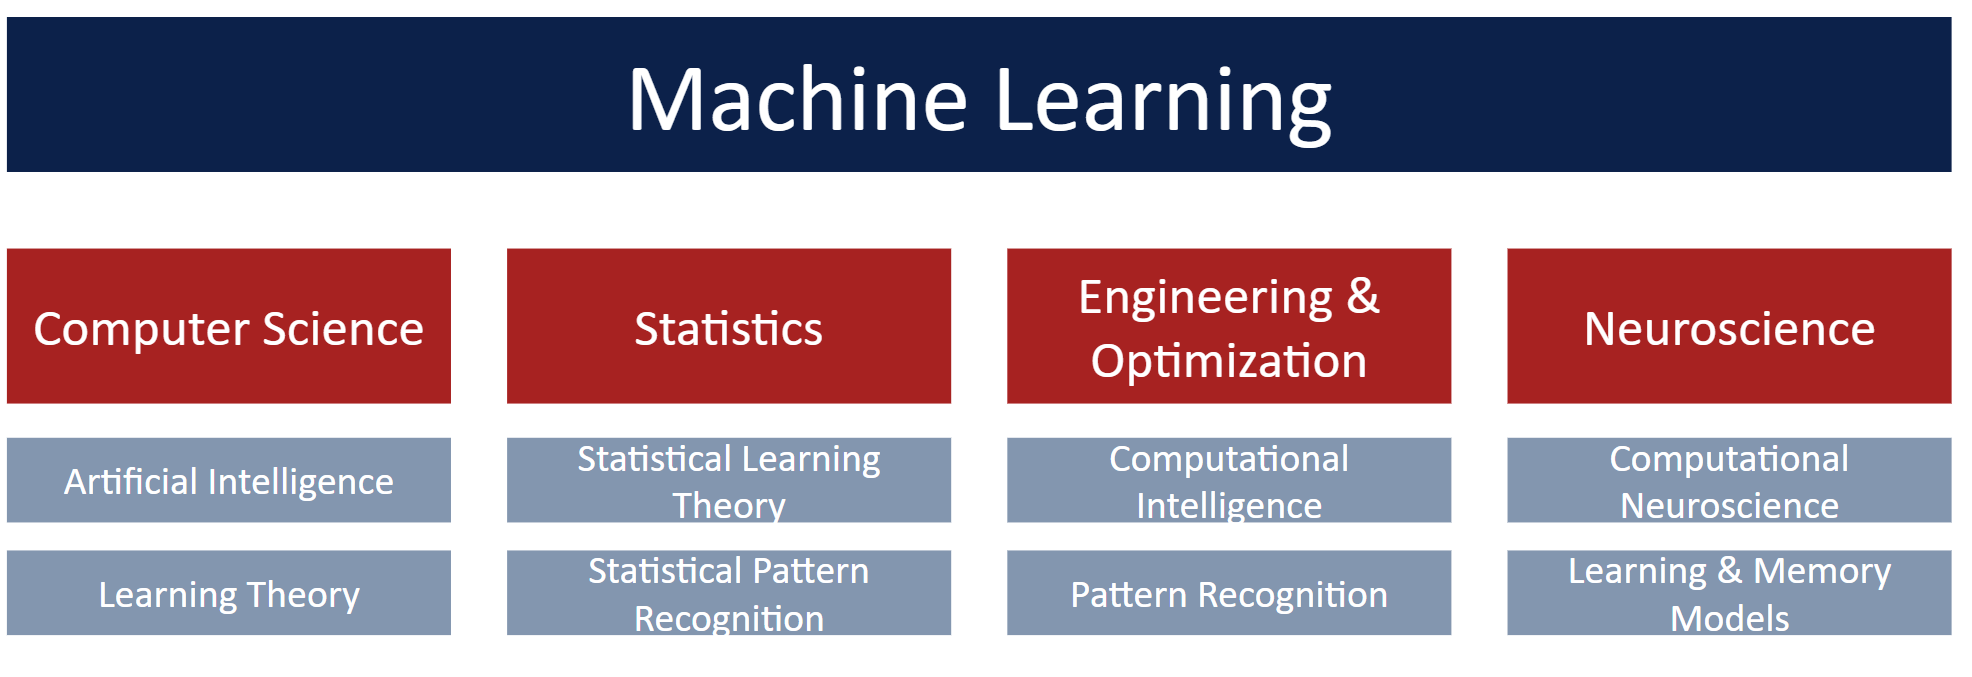
\includegraphics[width=.9\textwidth]{figures/intro-ml}
\end{center}
\end{frame}

\begin{frame}{}

\begin{center}

\Huge

\color{darkEmerald}

Is AI Machine Learning?

\end{center}

\end{frame}


\begin{frame}{}

\begin{center}

\Huge

\color{darkEmerald}

Is Data Science Machine Learning?

\end{center}

\end{frame}

%------------------------------------------------
\begin{frame}{Machine Learning, Data Science, Artificial Intelligence}
\begin{center}
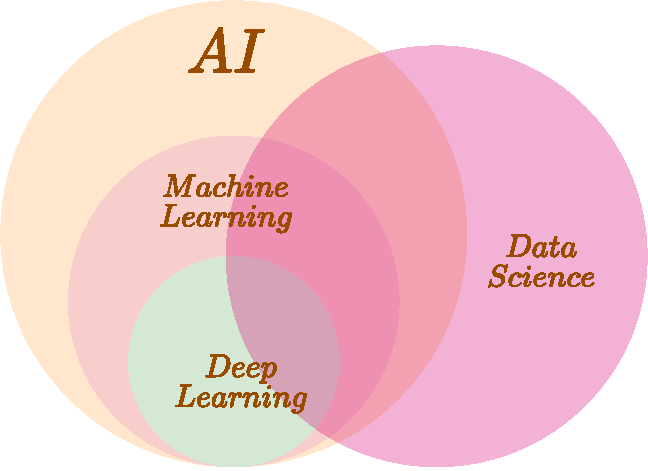
\includegraphics[height=.7\textheight]{figures/DI_ML_DL_DS.drawio.pdf}
\end{center}
\end{frame}

%------------------------------------------------
\begin{frame}{Milestones in AI}
\begin{center}
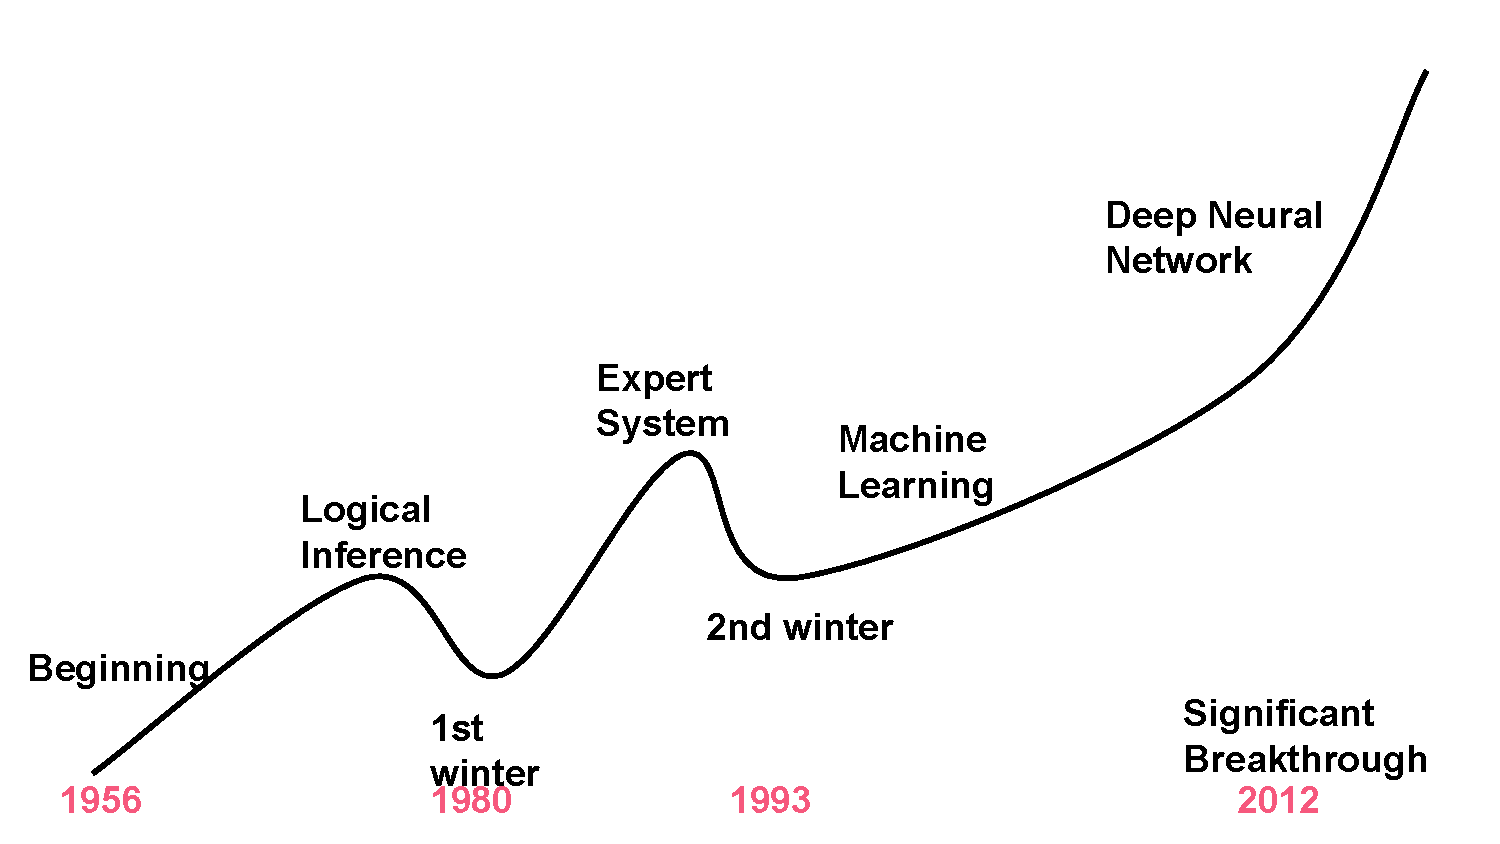
\includegraphics[width=.45\textwidth]{figures/AI_Trend.pdf}
\begin{texample}
First AI winter: AI cannot solve ‘combinatorial explosion’ problems

Second AI winter: expert system failed to scale


Reasons for AI winter: mismatch of expectations and technology gap
\end{texample}

\end{center}

\end{frame}

%------------------------------------------------
\begin{frame}{What's Different Now?}


\begin{columns}
    \column{0.5\linewidth}
    \begin{msgbox}{sageFuzz}{More Data}
        \begin{enumerate}
            \item Cheap storage
            \item  A lot more crowdsourced data: social media, android apps, data brokers
        \end{enumerate}
    \end{msgbox}

        \column{0.5\linewidth}
    \begin{msgbox}{mintCandy}{Better Algorithms}
        \begin{enumerate}
            \item Decades of research
            \item Key breakthrough: deep learning, attention-mechanism, transformers
        \end{enumerate}
    \end{msgbox}
\end{columns}

\begin{columns}
    \column{0.5\linewidth}
    \begin{msgbox}{hunterGreen}{Better Computing Stack}
        \begin{enumerate}
            \item GPU computation
            \item Cloud computing
        \end{enumerate}
    \end{msgbox}

        \column{0.5\linewidth}
    \begin{msgbox}{darkEmerald}{Investment and Mindset}
        \begin{enumerate}
            \item More investment and funding
            \item Larger pool of talents
        \end{enumerate}
    \end{msgbox}
\end{columns}

\end{frame}

\begin{frame}{}

  \begin{center}
    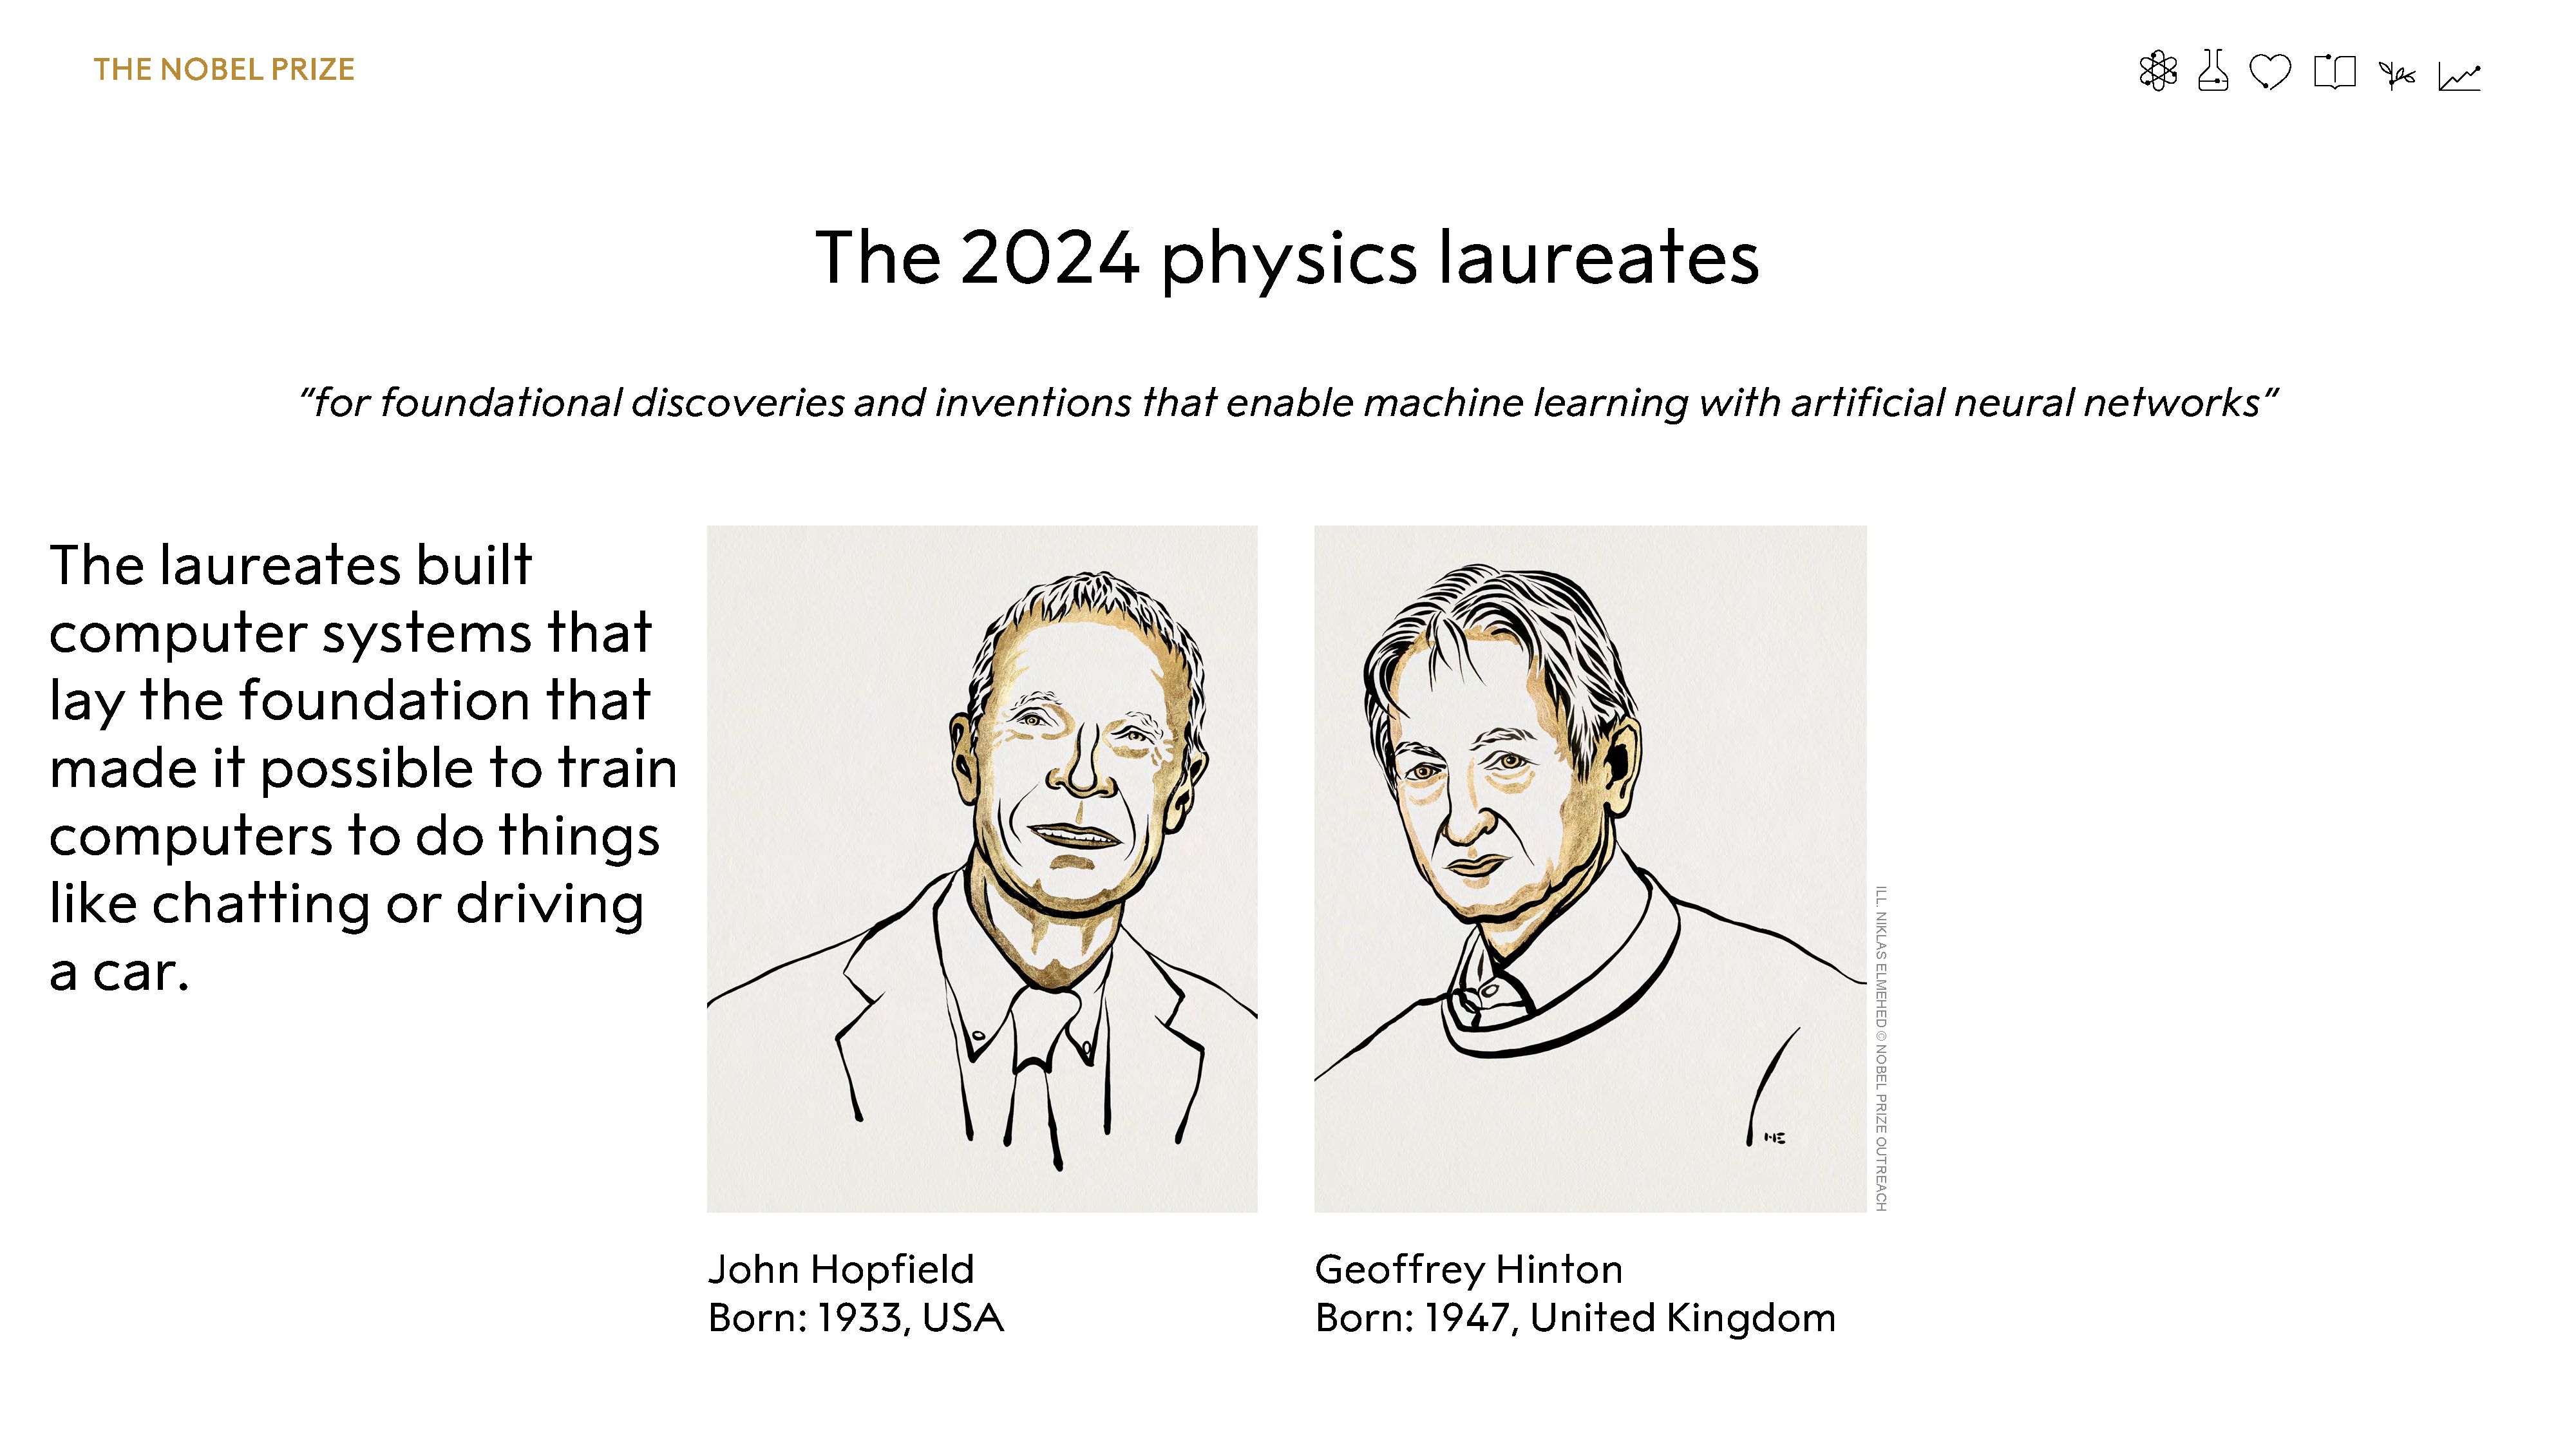
\includegraphics[width=.8\linewidth]{figures/nobel_physics_2024.pdf}  
    {\tiny Source: \url{https://www.nobelprize.org/uploads/2024/12/Slideshow_All_NobelPrizes_2024_NobelPrizeLessons.pdf}} 

  \end{center}
  
\end{frame}

%%%%%%%%%%%%%%%%%%%%%%%%%%%%%%%%%%%%%%%%%%%%%%%%%%%%%
\begin{subsectionframe}{What is possible with Machine Learning, Data Science and AI?}
\end{subsectionframe}


\begin{frame}{Big Data is Fueling AI}

\begin{center}
      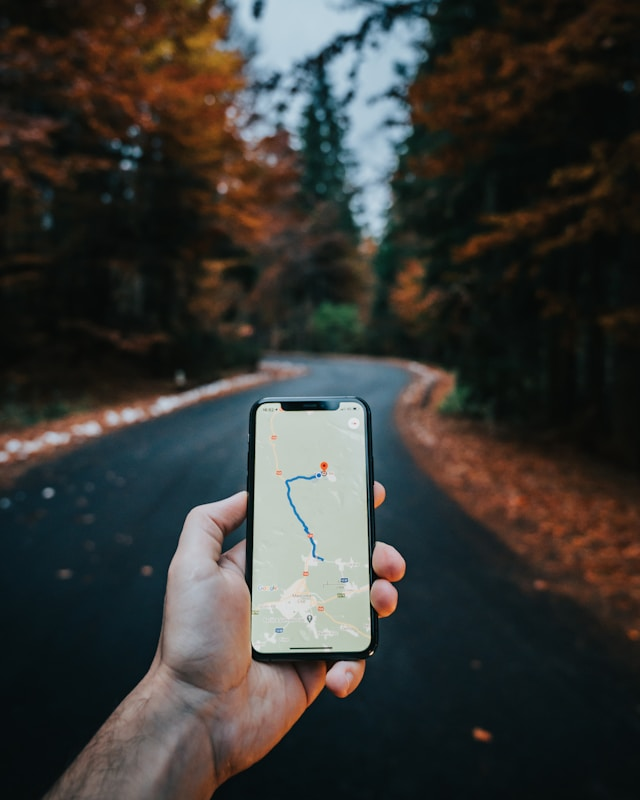
\includegraphics[height=.35\textheight]{figures/googlemap.jpg}
      
      Source: \url{https://unsplash.com/photos/person-holding-white-iphone-5-c-rEn-AdBr3Ig}
\end{center}
\begin{columns}
    \column{0.33\linewidth}
    \begin{redblock}{Previously}
        Best route by shortest path: no data-driven solution, no learning
    \end{redblock}

        \column{0.33\linewidth}
    \begin{redblock}{Now}
      Best route by current traffic: some form of data-driven solution
    \end{redblock}
    \column{0.33\linewidth}
    \begin{redblock}{Trending}
      Best route by predicted travel time: data-driven, learning-based solution
    \end{redblock}
\end{columns}
\end{frame}


\begin{frame}{Machine Learning Connecting Big Data and AI}
    \begin{center}
      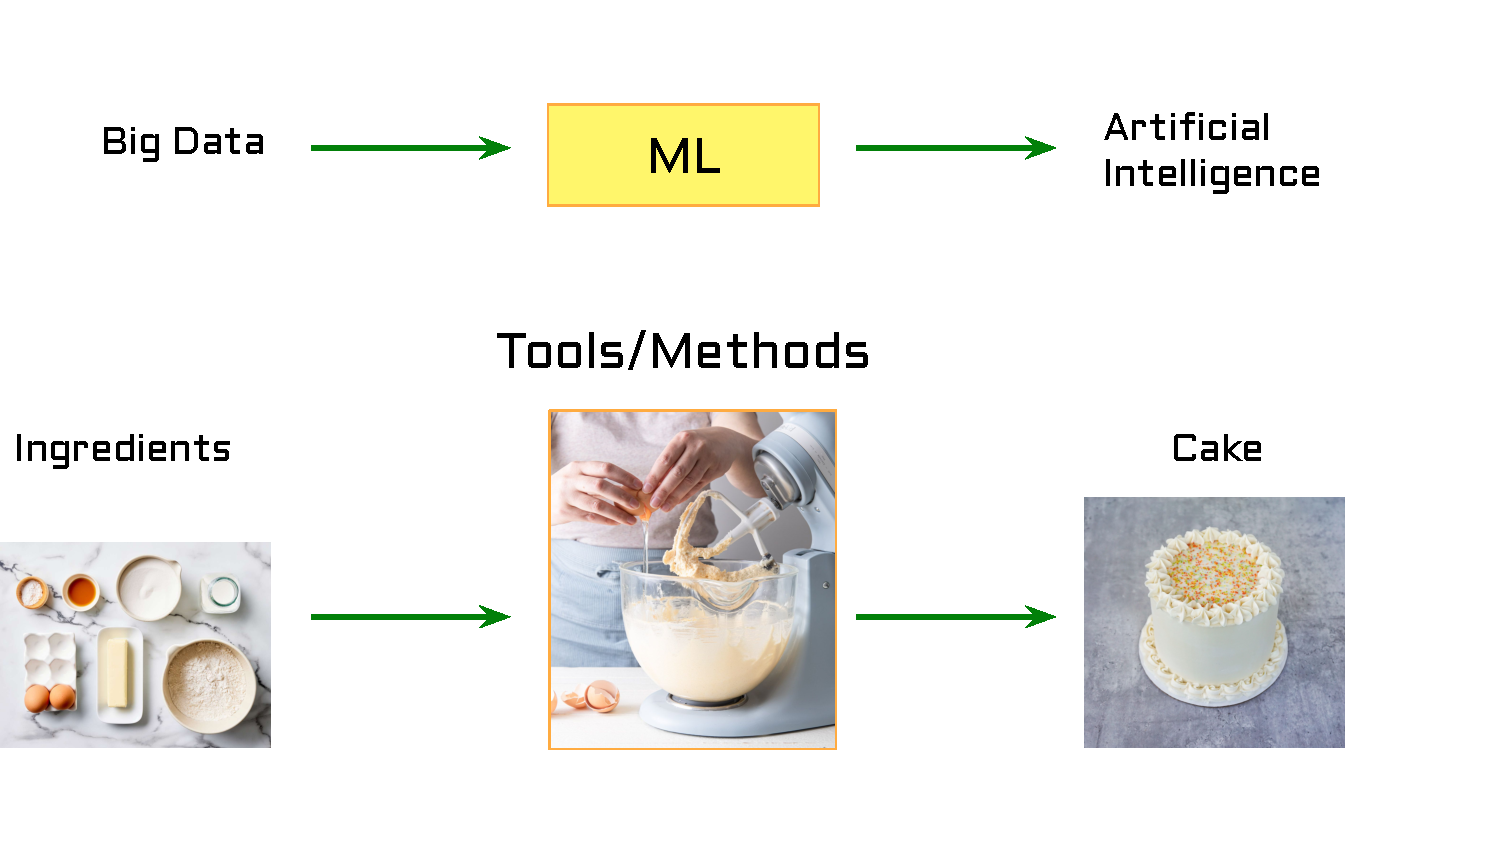
\includegraphics[height=.7\textheight]{figures/CakeData.pdf}
\end{center}
\end{frame}

\begin{frame}{Example of Prediction using Students' Records}
    \begin{center}
      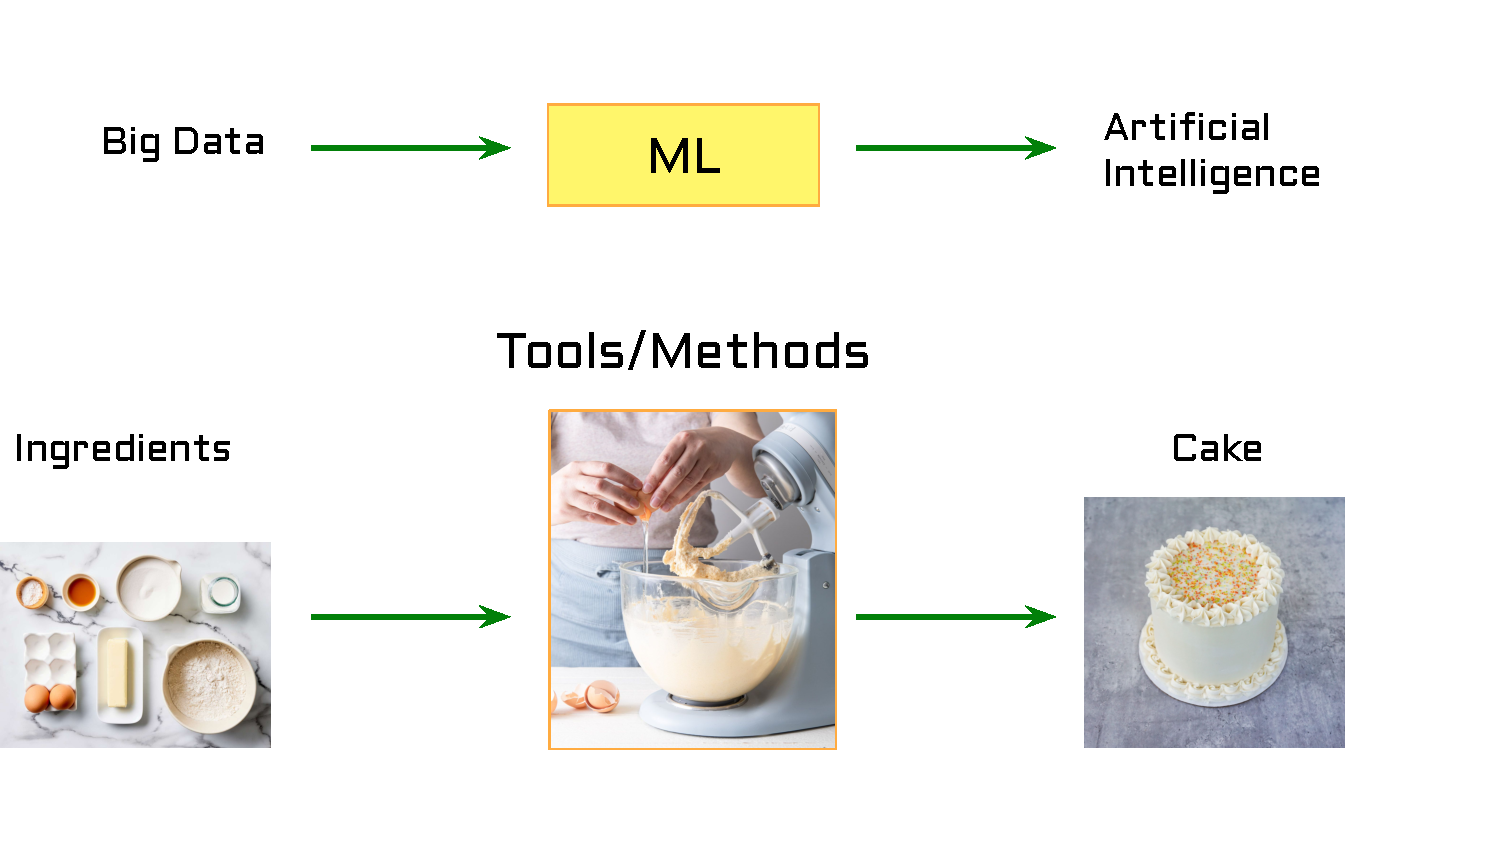
\includegraphics[width=0.7\linewidth,trim=0cm 10cm 0cm 0cm,clip]{figures/CakeData.pdf}
\end{center}
\begin{itemize}
    \item Data: Students’ records on quizzes
    \item AI: Predict if a student can answer correctly to another quiz question
\end{itemize}

 \begin{msgbox}{darkEmerald}{A Possible Solution using Machine Learning}
        \begin{enumerate}
            \item Give an ML model 10 million records from 5000 students
            \item ML determines strength and difficulty  of each students automatically, and make prediction about students' performance
        \end{enumerate}
    \end{msgbox}
    
\end{frame}




%------------------------------------------------
\begin{frame}{Broader Steps in Machine Learning}

\begin{itemize}
    \item \textbf{Explore: }
        \begin{itemize}
            \item Summarize
            \item Visualize
        \end{itemize}
    \item \textbf{Predict: }
    \begin{itemize}
        \item On Continuous Data
        \item On Categorical Data
    \end{itemize}
    \item \textbf{Simplify: }
    \begin{itemize}
        \item Group together based on common characteristics
        \item Model reduction
    \end{itemize}
    
\end{itemize}

\end{frame}



%------------------------------------------------
\begin{frame}{Text Prediction}
  \begin{center}\Large
    Given a word $\wbf(t)$ and some history $\hbf(t)$, what is the next word 
      (i.e., $\wbf(t+1)$)? What is the probability distribution over the next 
      word (i.e., $\Pbb(\wbf(t+1)|\wbf(t),\hbf(t))$)? \\
    \vspace{1em}
    
    \uncover<2->{\texttt{I love --?} } \\
    \uncover<3->{\texttt{Can you pick up milk at the --?} }
  \end{center}
\end{frame}





%------------------------------------------------
\begin{frame}{Optical Character Recognition}
  {\small\bf\color{MediumBlue}Bishop (2006)}
  \begin{center}
    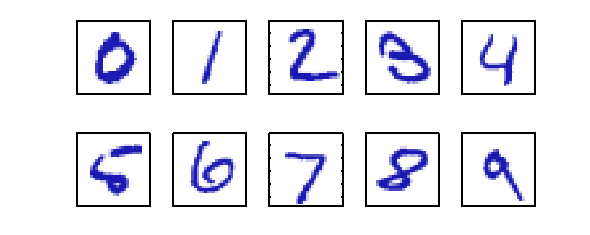
\includegraphics[width=\textwidth]{figures/intro-Figure11.pdf}\\
  \end{center}
\end{frame}


%------------------------------------------------
\begin{frame}{Prediction of Low/High Risk Loans}
  \begin{center}
    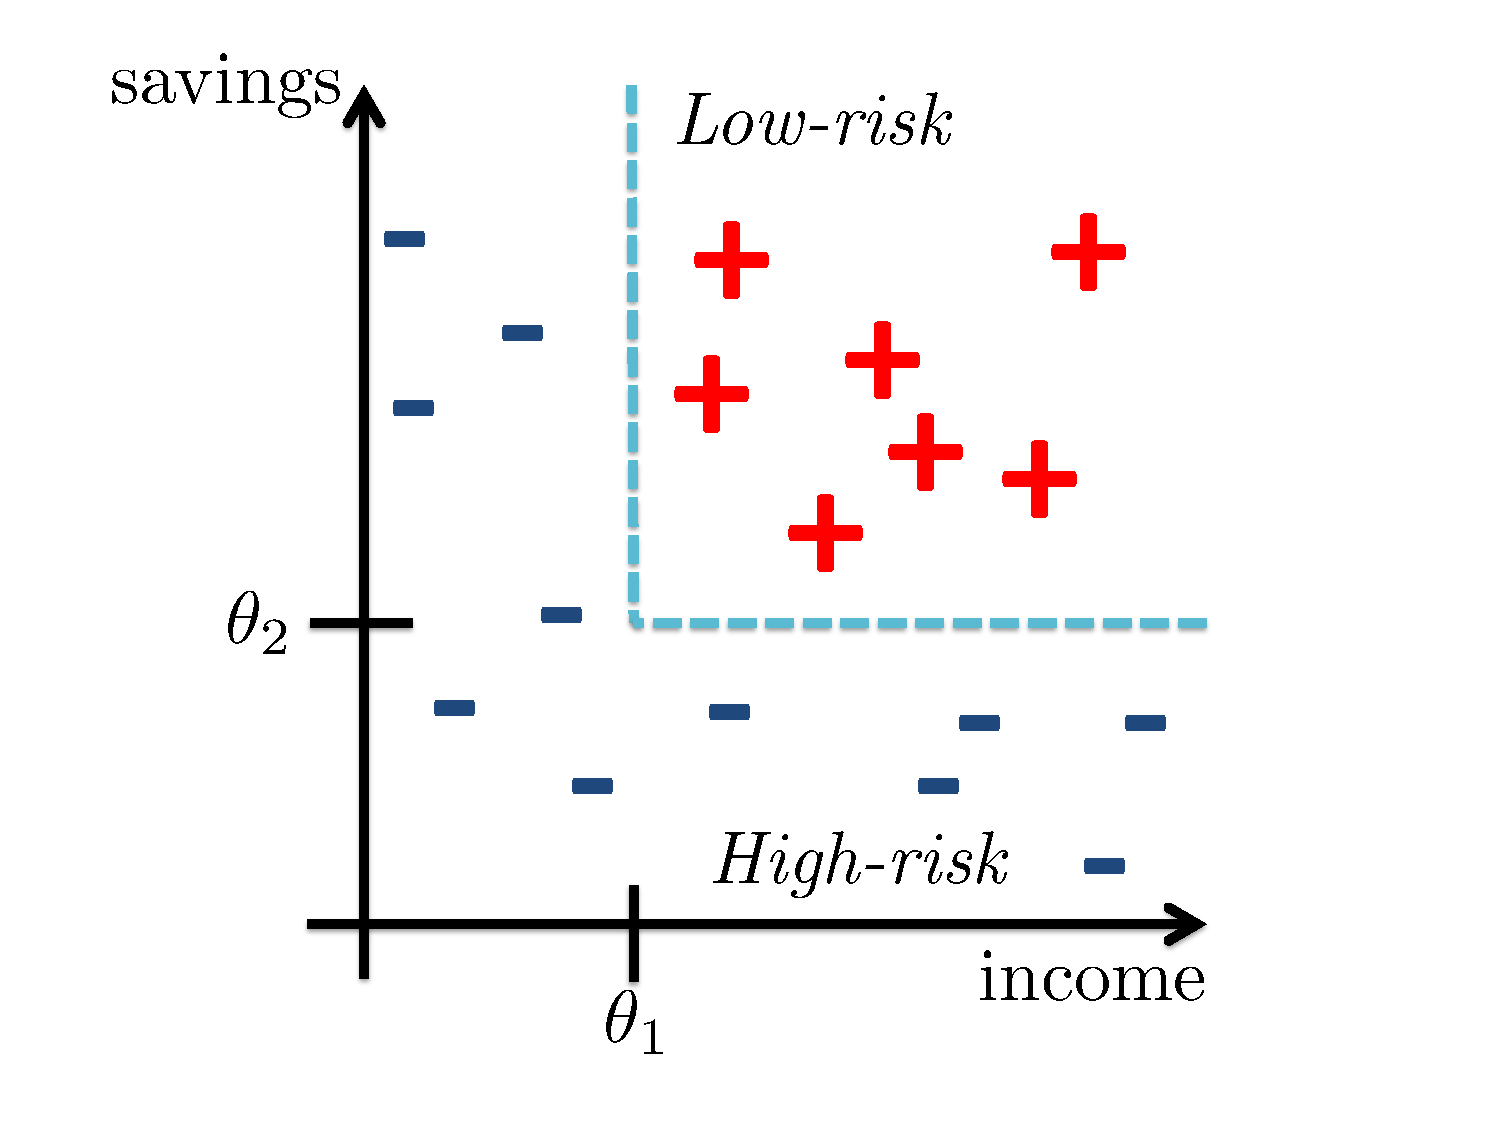
\includegraphics[height=.6\textheight]{figures/intro-loan.pdf}\\
    \texttt{if }($\textsf{income} > \theta_1$ AND $\textsf{savings} > \theta_2$) 
      \texttt{then} \{low-risk\} \texttt{else} \{high-risk\} 
  \end{center}
\end{frame}


%------------------------------------------------
\begin{frame}{Semiconductor}
  \begin{center}
    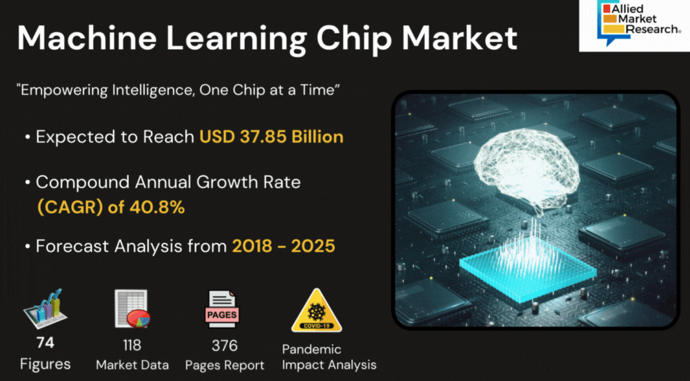
\includegraphics[width=.55\textwidth]{figures/semiconductor_AI.png}\\
    {\color{MediumRed}\url{https://www.linkedin.com/pulse/revolutionizing-tomorrow-unstoppable-rise-machine-learning-white-cyvef/}}
  \end{center}
\end{frame}


%------------------------------------------------
\begin{frame}{Drug Discovery and Medicine}

 \begin{columns}[c] 
\column{.49\textwidth} 
  \begin{center}
    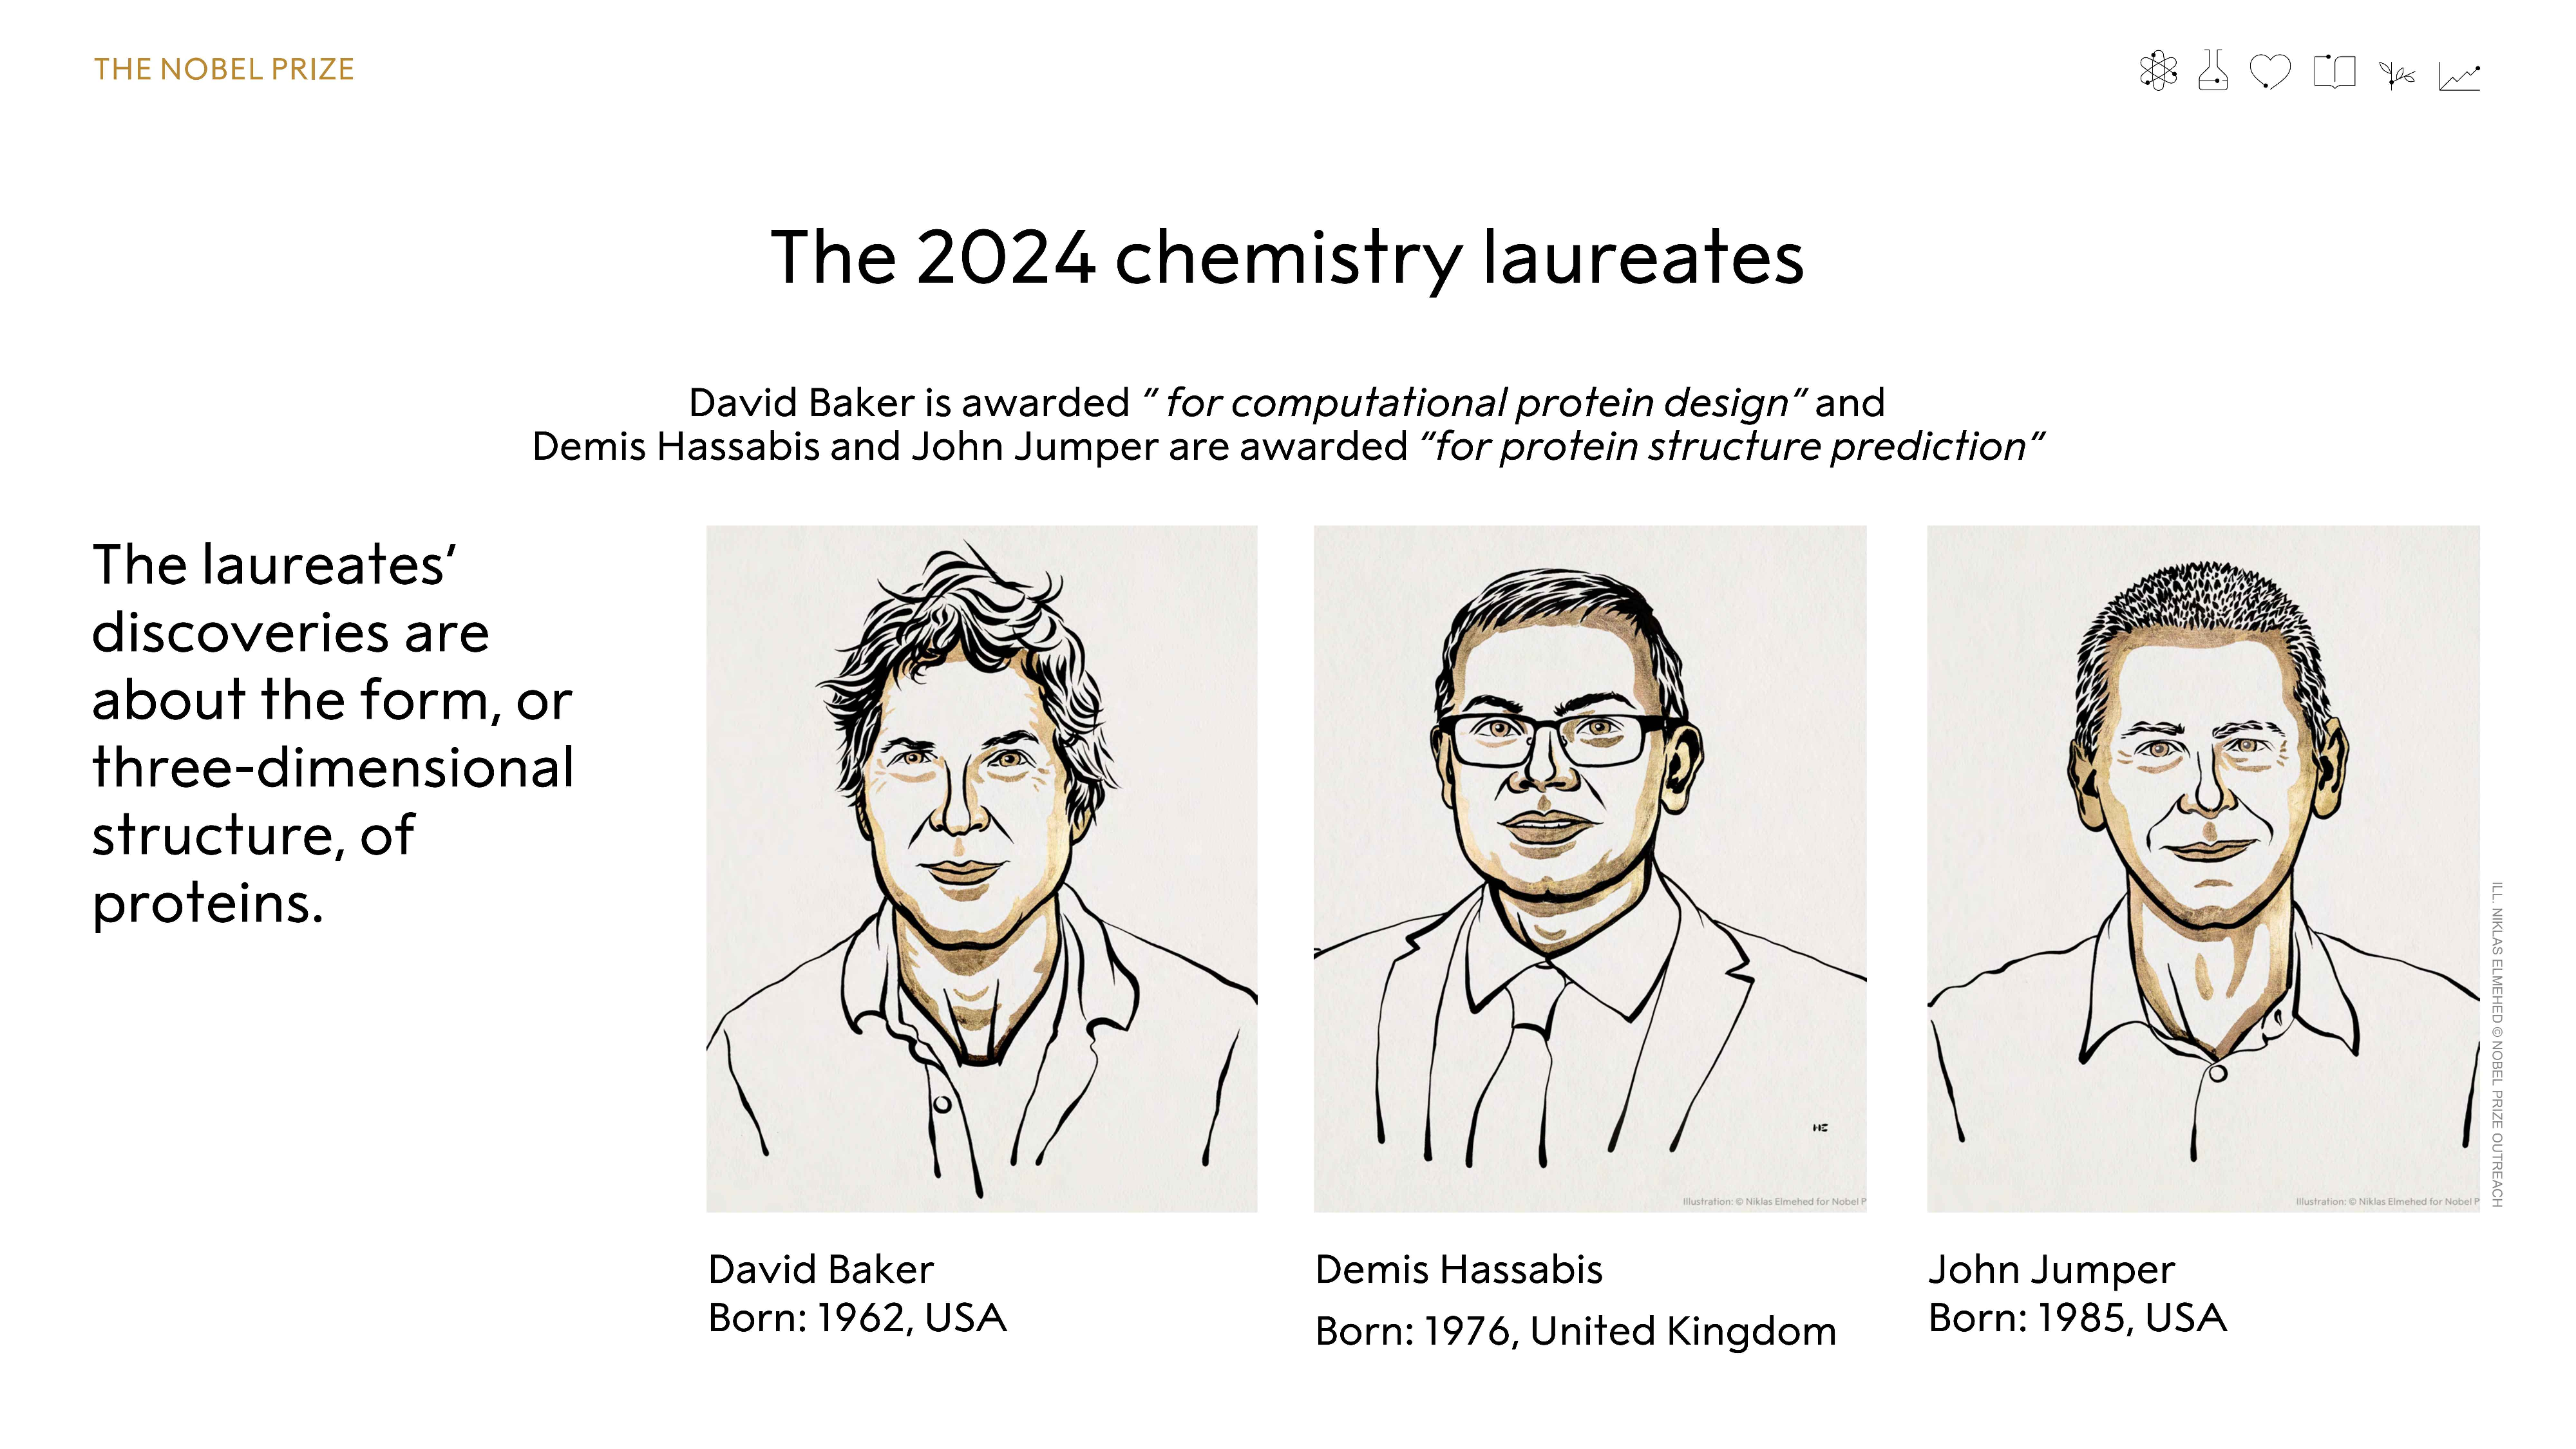
\includegraphics[width=.95\textwidth]{figures/nobel_physics_2024_alpha_fold_2.pdf}\\
     {\tiny\color{MediumRed}\url{https://www.nobelprize.org/uploads/2024/12/Slideshow_All_NobelPrizes_2024_NobelPrizeLessons.pdf}}
  \end{center}

\column{.49\textwidth} 
  \begin{center}
    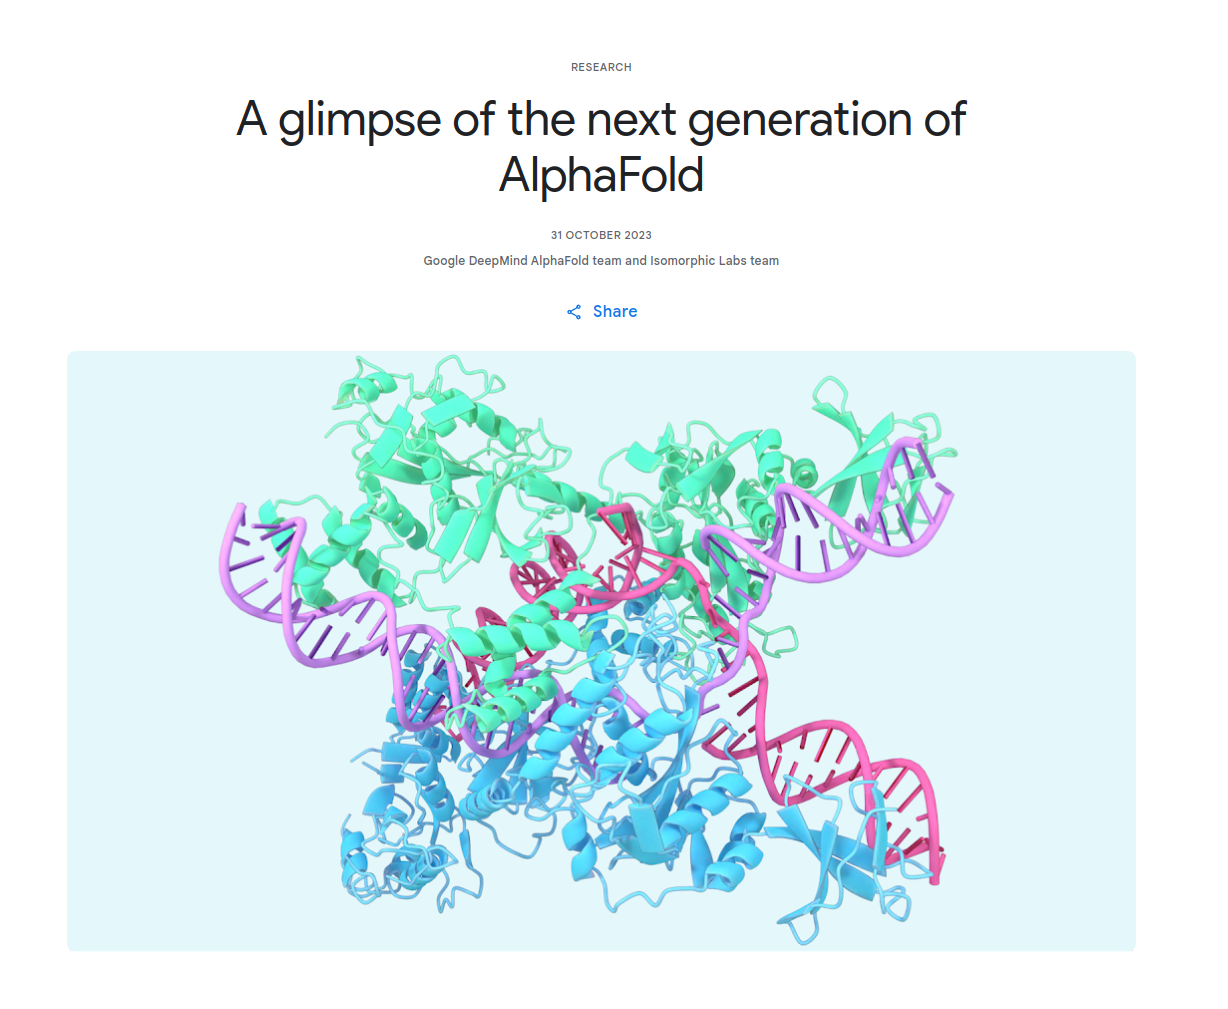
\includegraphics[width=.95\textwidth]{figures/alpha_fold.png}\\
     {\tiny Protein structure understanding and discovery: {\color{MediumRed}\url{https://deepmind.google/discover/blog/a-glimpse-of-the-next-generation-of-alphafold/}}}
  \end{center}
   \end{columns}
\end{frame}

%------------------------------------------------
% \begin{frame}{Finance}
%   \begin{center}
%     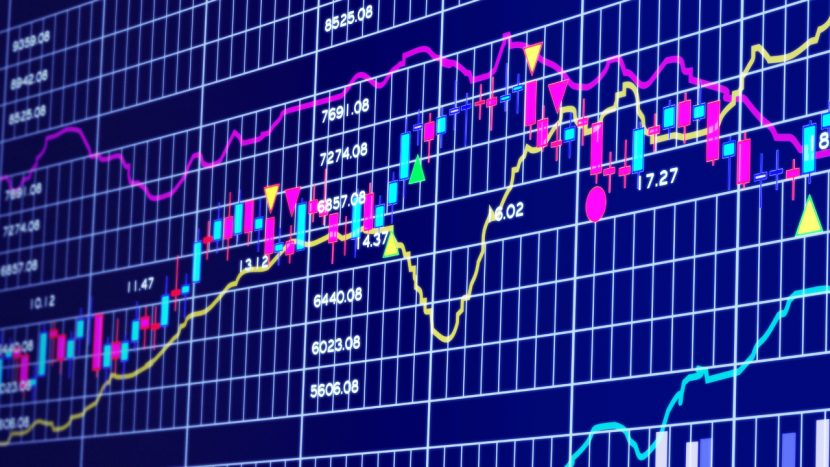
\includegraphics[width=.5\textwidth]{figures/intro-finance.jpg}\\
%   \end{center}
% \end{frame}

%------------------------------------------------
\begin{frame}{Intelligent Transportation}
  \begin{center}
    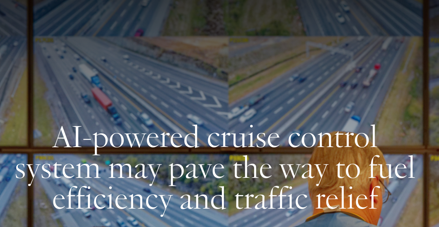
\includegraphics[width=.5\textwidth]{figures/transportation_AI.png}\\
    {\tiny\color{MediumRed}\url{https://news.vanderbilt.edu/2022/11/23/ai-powered-cruise-control-system-may-pave-the-way-to-fuel-efficiency-and-traffic-relief/}}
  \end{center}
\end{frame}

%------------------------------------------------
\begin{frame}{What is Machine Learning}
\begin{tblock}{An Informal Definition}
Automated analysis of – typically large volumes of – data in search of hidden structures / patterns / information
\begin{itemize}
    \item<2-> {\bf\color{DarkBlue} Pattern recognition}: Classification of objects into (predefined) categories or classes 
    \begin{itemize}
        \item Given data, assign labels (categories) that identify the correct class 
        \item Identify the input/output relationship (mapping) of an unknown system (system identification) 
    \end{itemize}
    \item<3-> {\bf\color{DarkBlue} Mathematically}: $f: \Xcal \mapsto \Ycal$. How are we going to find $f(\x)$?
\end{itemize}
\end{tblock}
\end{frame}


%------------------------------------------------
\begin{frame}{What is Data Mining}
\begin{tblock}{Precursor to Machine Learning}
Process of identifying valid, novel, potentially useful, and ultimately understandable patterns in data
\begin{itemize}
    \item<2-> Extract previously unknown, comprehensible, and actionable information from large databases and use it to make crucial business decisions
    \item<3-> A set of methods used in the knowledge discovery process
    \item<4-> Discover advantageous patterns in data
    \item<5-> A decision support process where we look in large databases
for unknown and unexpected patterns of information
\end{itemize}
\end{tblock}
\end{frame}


\section{Machine Learning in Era of Large Language Models}

\begin{frame}
    \sectionpage
\end{frame}

\begin{frame}{How to Machine Learning with LLMs!}

\begin{center}\
\huge
\color{nuaablue}
LLMs are as good as you can think!\footnote{With Some Caution!}
\end{center}
\end{frame}

\begin{frame}{Learning to Learn}

\begin{center}\

\huge

\color{nuaablue}

How to learn is even more important now! 

\large

\begin{enumerate}



\item What to ask!
\item Ask better questions
\item How do I know if the response from LLMs are correct?
\item Can I stop learning to code? Then why am I learning Machine Learning?

\end{enumerate}

\end{center}


\end{frame}


%------------------------------------------------
\begin{frame}{Types of Learning}
\begin{tblock}{Learning Modalities}
    
\begin{itemize}
    \item<2-> {\bf\color{DarkBlue} Supervised learning}: Given training data with previously labeled classes, learn the mapping between the data and their correct classes. 
    \item<3-> {\bf\color{DarkBlue} Unsupervised learning}: Given unlabeled data obtained from an unknown number of categories, learn how to group such data into meaningful clusters based on some measure of similarity
    \item<4-> {\bf\color{DarkBlue} Reinforcement learning}: Given a sequence of outputs, learn a policy to obtain the desired output game-playing problems.
\end{itemize}
\end{tblock}

\end{frame}

\begin{frame}{Machine Learning for Modern AI}
     \begin{center}
    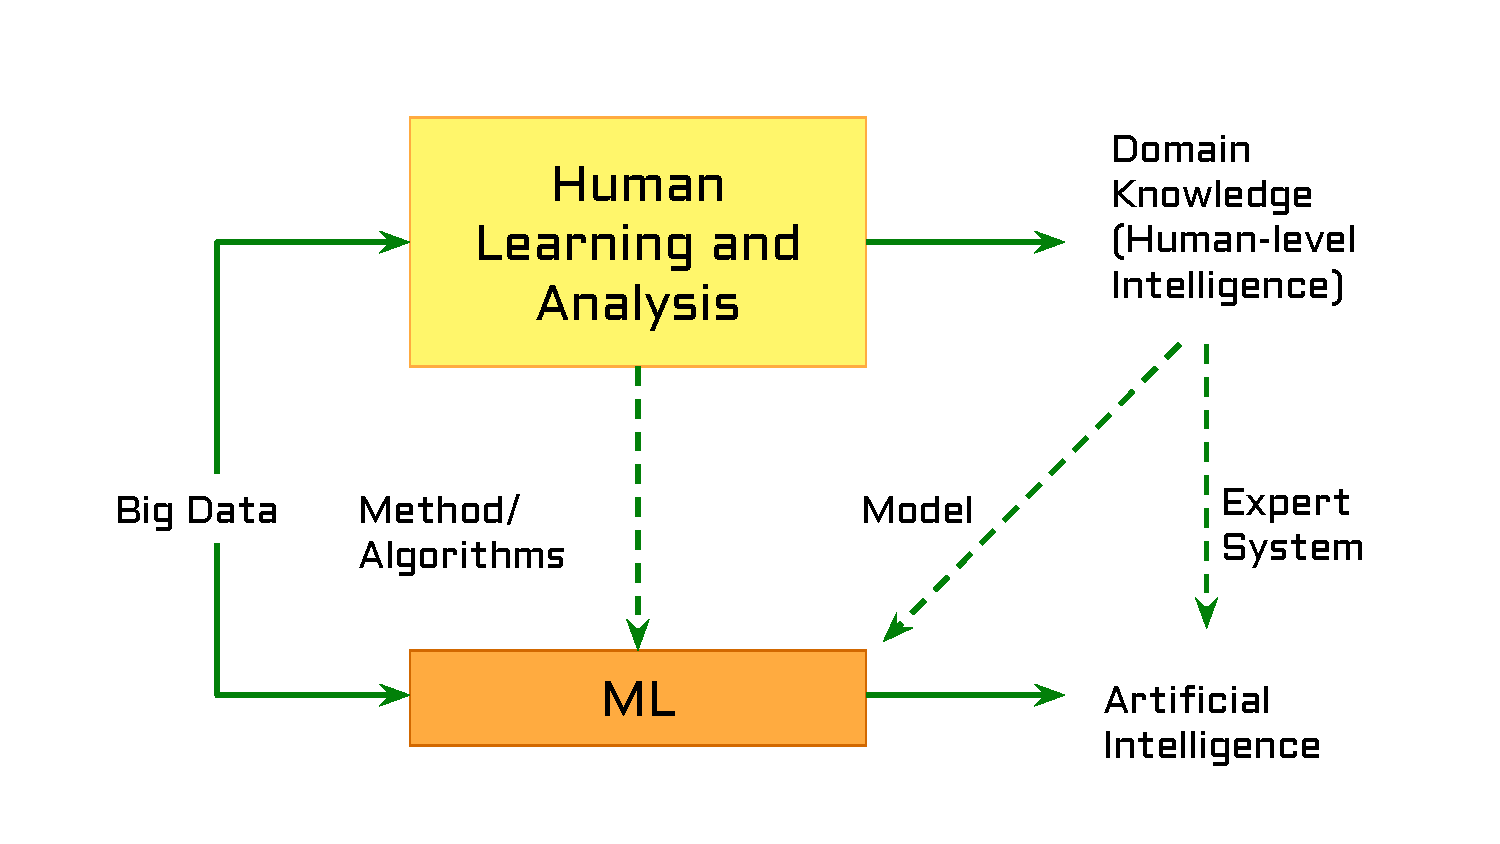
\includegraphics[width=0.42\linewidth,trim=1cm 1.5cm 1cm 1.5cm,clip]{figures/ModernAI.pdf}
  \end{center}
  \begin{columns}
    \column{0.5\linewidth}
    \begin{redblock}{Human Learning}
        \begin{enumerate}
            \item Subjective
            \item Domain knowledge generation
            \item Fast basic solution
        \end{enumerate}
    \end{redblock}

        \column{0.5\linewidth}
    \begin{redblock}{Machine Learning}
      \begin{enumerate}
            \item Objective
            \item Harness computing power
            \item Incremental improvement
        \end{enumerate}
    \end{redblock}
\end{columns}
\end{frame}

\begin{frame}{Generative Artificial Intelligence /Generative ML}
\begin{columns}
    \column{0.33\linewidth}
    \begin{enumerate}
    \item Pattern Recognition
    \begin{itemize}
        \item Listen/Read/Watch
    \end{itemize}
    \item Generative ML
    \begin{itemize}
        \item Speak/Write/Draw
    \end{itemize}
\end{enumerate}

        \column{0.33\linewidth}
    Variations:
    
        \vspace{2pt}
    
            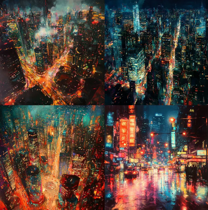
\includegraphics[width=0.86\linewidth,trim=1cm 1.5cm 1cm 1.5cm,clip]{figures/genAI4.png}

 \column{0.33\linewidth}
   Style change:
   
        \vspace{2pt}
        
            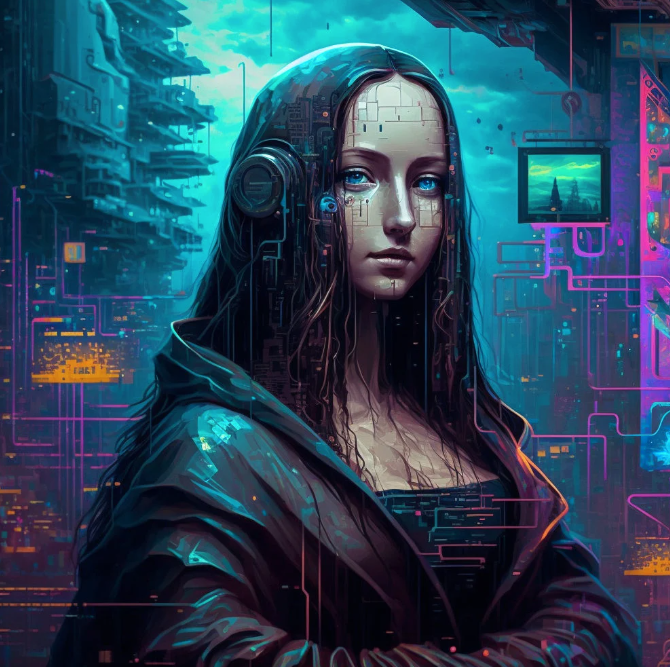
\includegraphics[width=0.9\linewidth,trim=1cm 1.5cm 1cm 1.5cm,clip]{figures/Cyberpunk_Mondalisa.png}
    
\end{columns}


    
\end{frame}

\begin{frame}{Example of Learning Problems}
\begin{itemize}
    \only<1> {\item Forecast the spread of disease (Regression): Using health records, demographic data, and travel patterns, predict the spread of a disease like COVID-19.
    \begin{center}
      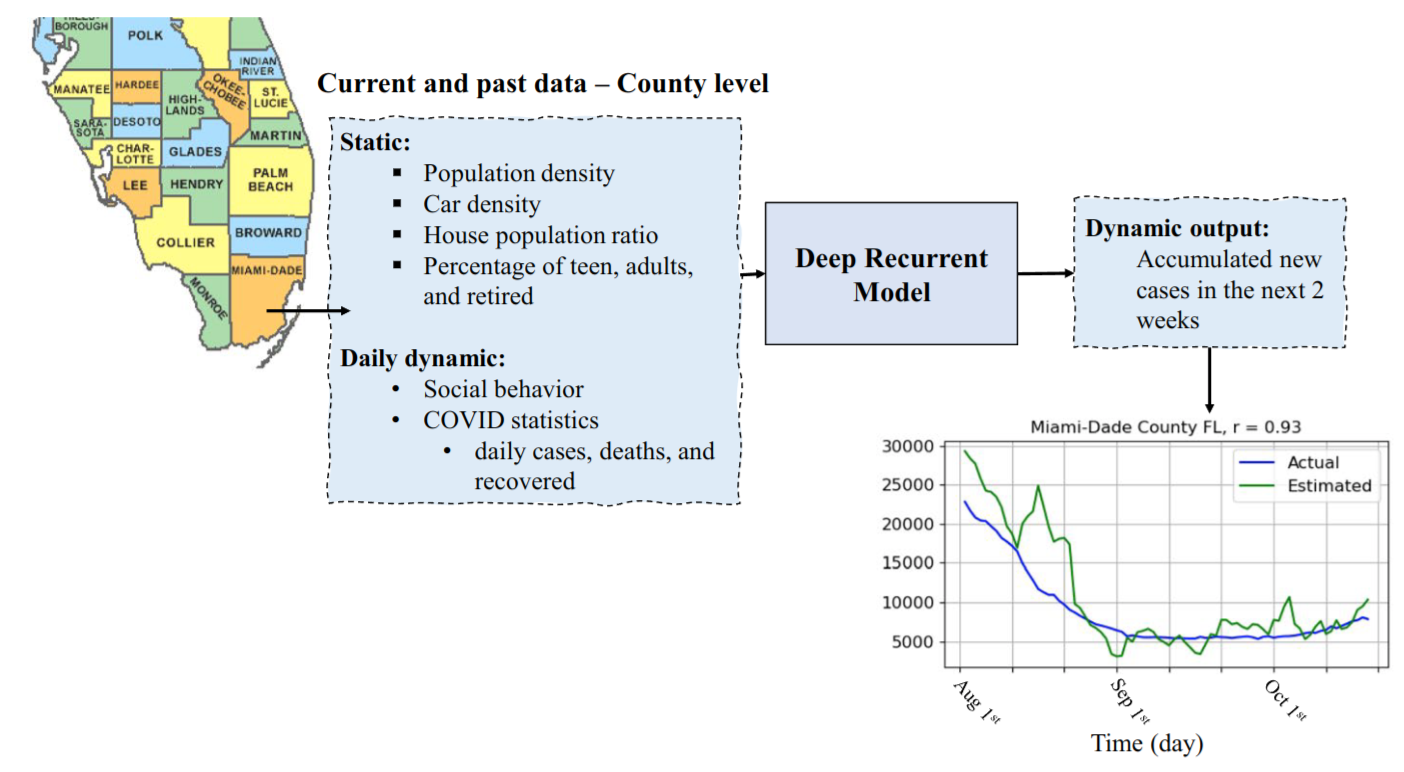
\includegraphics[width=0.6\linewidth]{figures/COVID_Forecast.png}
      {\tiny From paper: \bf The forecast of COVID‑19 spread risk
      at the county level}
    \end{center}
    }
    \only<2> {\item Identify fraudulent credit card transactions (Classification): Based on transaction details, customer behavior, and historical fraud patterns, build a model to predict whether a new transaction is likely to be fraudulent.}
    \only<3> {\item Predict the impact of climate change on crop yields (Regression): Using climate models, historical weather data, and crop yield records, predict how climate change will affect crop yields in different regions.
    \begin{center}
      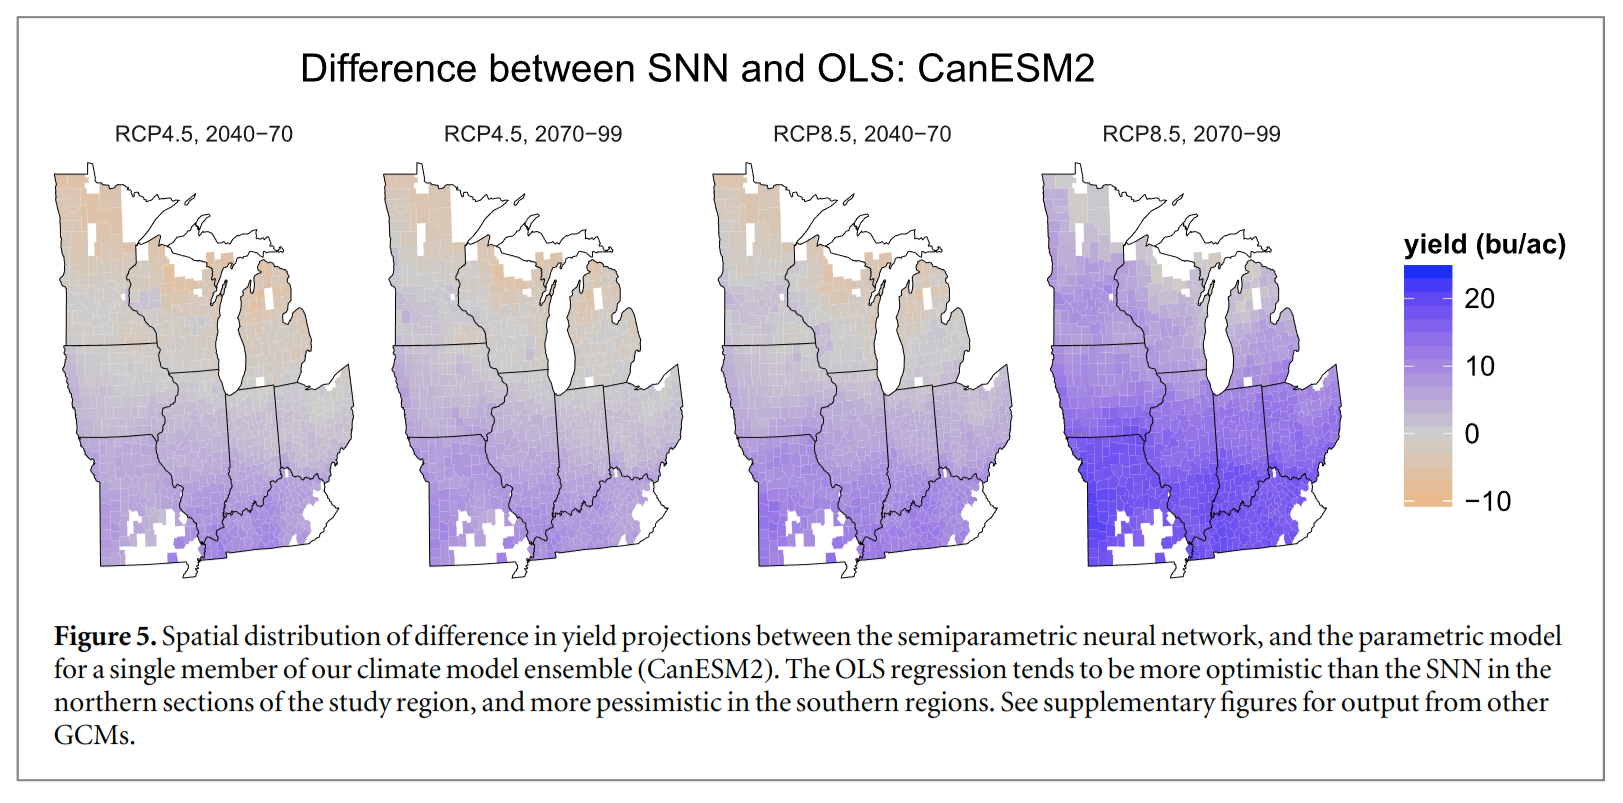
\includegraphics[width=0.6\linewidth]{figures/crop_yield.png}

      {\tiny From paper: \bf Machine learning methods for crop yield prediction and climate change impact assessment in agriculture}
    \end{center}
    }
    \only<4>{ \item Predict the failure of a mechanical component (Classification): Based on operational data and component characteristics, predict whether a mechanical component will fail in the next cycle.}
    \only<5> {\item Predict the efficiency of a power plant (Regression): Based on operational data and environmental conditions, predict the efficiency of a power plant.}

     \only<6> { \item  Optimize the operation of a supply chain (Optimization): Using historical data and predictive models, optimize the operation of a supply chain to minimize cost and maximize efficiency.}
    \only<7> { \item Predict the traffic flow in a city (Regression): Using historical traffic data, weather data, and event information, predict the traffic flow in a city.}
   \only<8> {  \item Predict the load on a power grid (Regression): Based on weather data, time of day, and historical load data, predict the load on a power grid.}
    \only<9> { \item Traffic signal timing (Reinforcement Learning): Optimize the timing of traffic signals in a city to minimize traffic congestion and improve traffic flow.}
  \only<10> {   \item Optimal bidding in energy markets (Reinforcement Learning): Determine the optimal bidding strategy in energy markets to maximize profit.}

    
\end{itemize}

\end{frame}

 %------------------------------------------------
 \begin{frame}{Supervised Learning}

 \begin{center}
     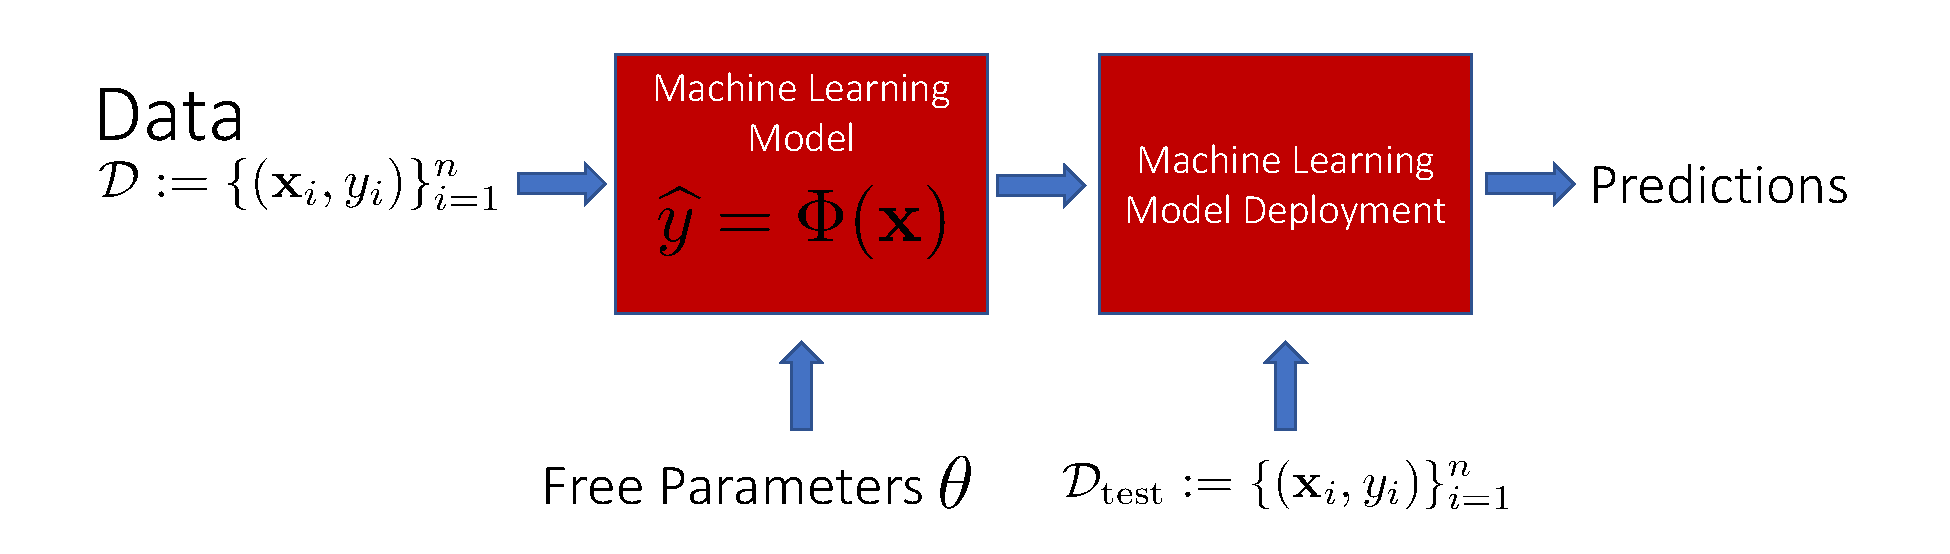
\includegraphics[height=.5\textheight]{figures/ml.pdf}
 \end{center}

 \end{frame}


 \begin{frame}
   \frametitle{Unsupervised Learning}
    \begin{center}
    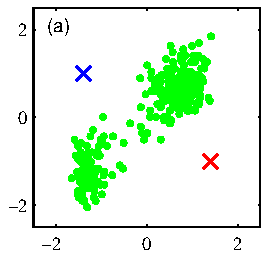
\includegraphics[scale=.4]{figures/Figure91a.pdf}
    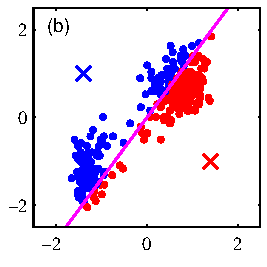
\includegraphics[scale=.4]{figures/Figure91b.pdf}
    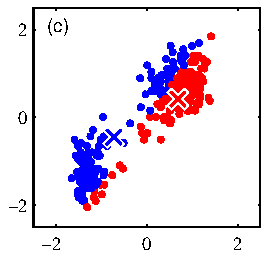
\includegraphics[scale=.4]{figures/Figure91c.pdf} \\
    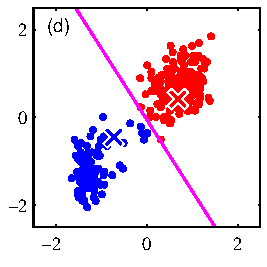
\includegraphics[scale=.4]{figures/Figure91d.pdf}
    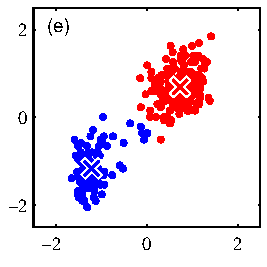
\includegraphics[scale=.4]{figures/Figure91e.pdf}
    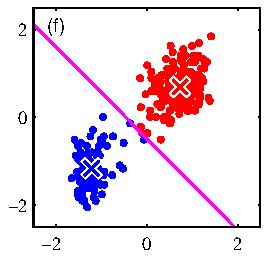
\includegraphics[scale=.4]{figures/Figure91f.pdf} \\
    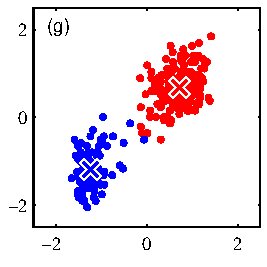
\includegraphics[scale=.4]{figures/Figure91g.pdf}
    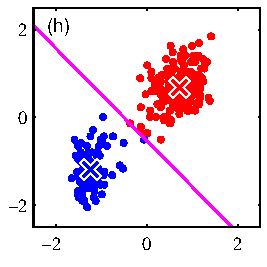
\includegraphics[scale=.4]{figures/Figure91h.pdf}
    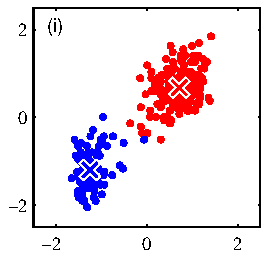
\includegraphics[scale=.4]{figures/Figure91i.pdf}
    \end{center}
 \end{frame}

% %------------------------------------------------
 \begin{frame}{Reinforcement Learning}
   \begin{center}
     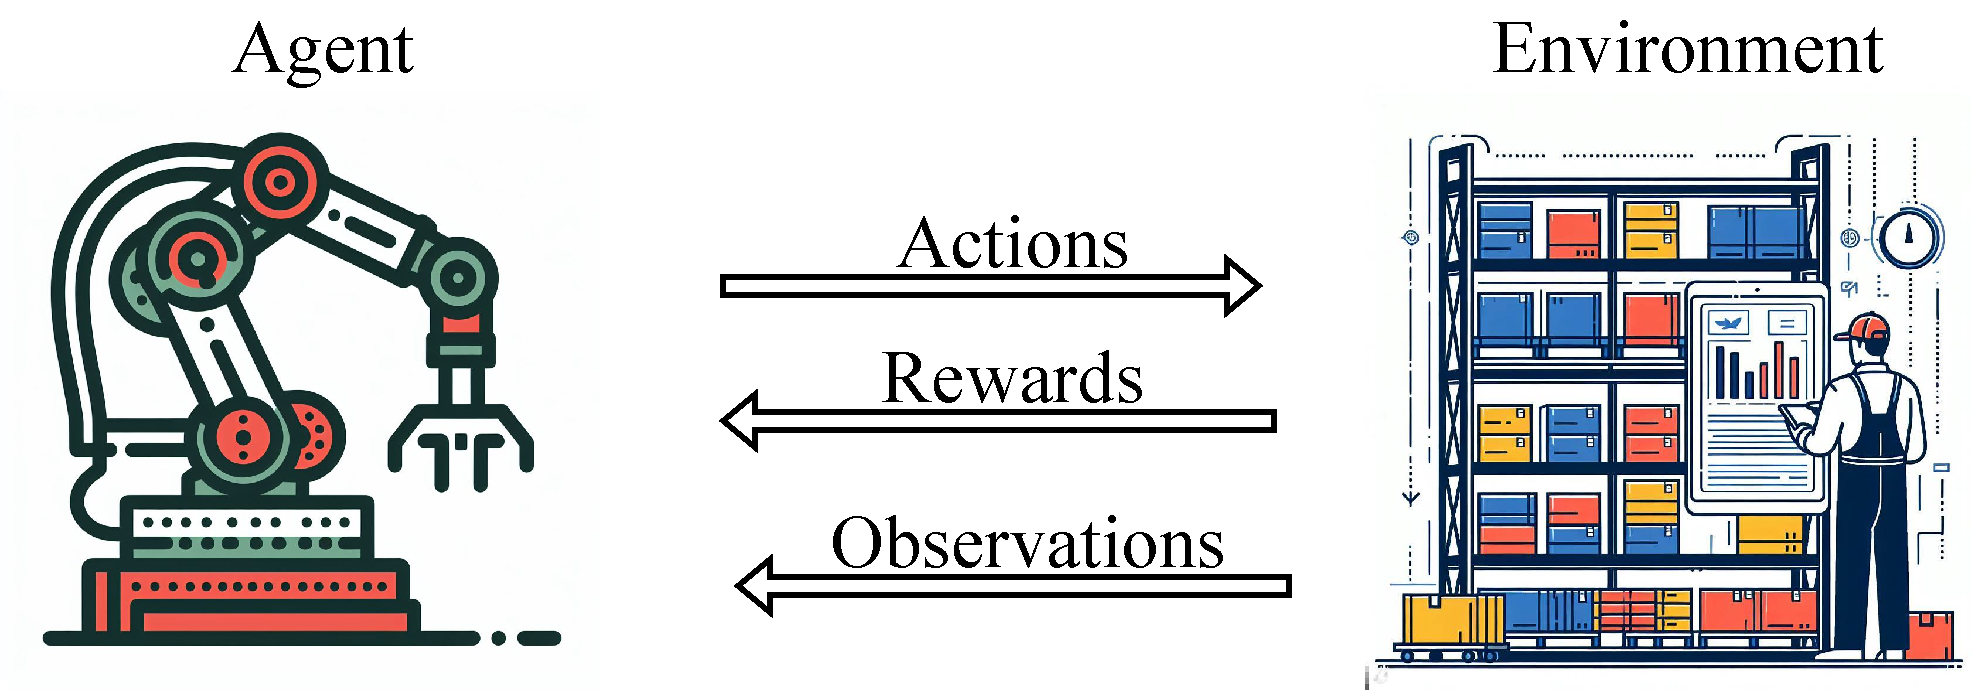
\includegraphics[width=.8\textwidth]{figures/rl_robot.drawio.pdf}\\
   \end{center}
 \end{frame}


 %------------------------------------------------
 \begin{frame}
   \frametitle{\bf Terminology}
   \begin{itemize}
 \only<1> {    \item {\color{MediumBlue}Feature}: a variable, $x$, believed to carry information about the task. {\em example}, cholesterol level.}

 \only<2> {    \item {\color{MediumBlue}Feature vector}: collection of variables, or features, $\xbf = [x_1,\ldots,x_D]^\T$. {\em example}, collection of medical tests for a patient.}

  \only<3> {   \item {\color{MediumBlue}Feature space}: $D$-dimensional vector space where the vectors $\xbf$ lie. {\em example}, $\xbf \in \Rbb_+^D$}
 
  \only<4> {   \item {\color{MediumBlue}Class}: a category/value assigned to a feature vector. in general we can refer to this as the target variable ($t$). {\em example}, $t = \textrm{cancer}$ or $t = 10.2\,^{\circ}\mathrm{C}$.}
 
 \only<5> {    \item {\color{MediumBlue}Pattern}: a collection of features of an object under consideration, along with the correct class information of that object defined by, $\{\xbf_n,t_n\}$.}

  \only<6> {   \item {\color{MediumBlue}Training data}: data used during training of a classifier for which the correct labels are {\em a priori} known.}
 
  \only<7> {   \item {\color{MediumBlue}Testing/Validation Data}: data not used during training, but rather set aside to estimate the true  (generalization) performance of a classifier, for which correct labels are also a priori known.}
 
  \only<8> {   \item {\color{MediumBlue}Cost Function}: a quantitative measure that represents the cost of making an error. a model is produced to minimize this function. Is zero error always a good thing?}
 
  \only<9> {   \item {\color{MediumBlue}Classifier}: a parametric or nonparametric model which adjusts its parameters or weights to find the mapping from the feature space to the outcome (class) space. $f: \Xcal \mapsto \Tcal$. 
       \begin{itemize}
         \item $y(\xbf) = \wbf^\T\xbf + b$
         \item $\ybf(\xbf) = \sigma(\Wbf^\T \xbf + \bbf)$ where $\sigma$ is a soft-max
         \item $\ybf(\xbf) = \sigma( \Qbf^\T\nu(\Wbf^\T \xbf + \bbf) +\qbf )$ where $\sigma$ is a soft-max and $\nu$ is a sigmoid
         \item We need to optimize parameters $\Qbf$, $\Wbf$, $\wbf$, $\bbf$, $\qbf$ and/or $b$ to minimize a cost 
       \end{itemize}}
      
 \only<10> {    \item {\color{MediumBlue}Model}: a simplified mathematical/statistical construct that mimics (acts like) the underlying physical phenomenon that generated the original data.}
   \end{itemize}
 \end{frame}


%%%%%%%%%%%%%%%%%%%%%%%%%%%%%%%%%%%%%%%%%%%%%%%%%%%%%
\begin{subsectionframe}{Machine Learning for AI in Reality}
\end{subsectionframe}


\begin{frame}{Frequently Asked Questions on ML for AI}

\begin{itemize}


 \only<1> {  
 \item 
 Finding AI Projects $\approx$ Find a research topic
 \begin{itemize}
\item  Motivation: what are you interested in?
\begin{itemize}
\item Something to publish?
\item Something than can improve performance of xyz?
\item Something that may lead to deeper study and novel insights?
\end{itemize}
 \item Feasibility: what can or cannot be done? 
 \begin{itemize}
 \item Modeling
 \item Computation
 \item Budget
 \item Timeline
 \end{itemize}
 \end{itemize}
 }



\only<2>{
\item What is the best machine learning model for the given data and AI?

\begin{tblock}{Answer}
We don't know, I don't know, requires exploration, but perhaps start with simpler models.

\end{tblock}
}

\only<3>{
\item Myth: AI works best with the sophisticated models
\begin{tblock}{Response}
Sophisticated models:
\begin{itemize}
\item time-consuming to train and predict
\item difficult to tune or modify
\item  hard to ``simplify" nor ``analyze"
\end{itemize}
\end{tblock}
A simpler models should be the first choice.
}


\only<4>{
\item Simpler model first
\begin{tblock}{Keep it simple and safe}
\begin{itemize}
\item Easy to train and predict
\item Easy to tune parameters and modify
\item Easy to analyze
\item Smaller risk
\end{itemize}
\end{tblock}

}

\end{itemize}




\end{frame}


\begin{frame}{Planning your Machine Learning Project}

\begin{columns}
\column{0.33\linewidth}

\begin{tblock}{Data}
\begin{itemize}
\item Data collection
\item Data cleaning
\item Data storing 
\item ~ $\vdots$
\end{itemize}
\end{tblock}


\column{0.33\linewidth}


\begin{tblock}{Methods}

\begin{itemize}
\item Modeling
\item Computation
\item Applying other non-ML techniques
\end{itemize}

\end{tblock}




\column{0.33\linewidth}

\begin{tblock}{End-use}
\begin{itemize}
\item Evaluation
\item Deployment
\item User-interface
\item Scalability
\end{itemize}

\end{tblock}



\end{columns}

\begin{texample}
A necessary first step: set up an evaluation criteria
\end{texample}

\end{frame}


%------------------------------------------------
\begin{frame}{What do you need to be successful in this course?}
\begin{itemize}
    \item<2-> {\bf\color{MediumBlue}Linear Algebra}: Data are represented as vectors, vectors lie in a vector space, \ldots, you get the point!
      \item<3-> {\bf\color{MediumBlue}Calculus}: A little bit of calculus is needed to understand  how optimization problem works!
    \item<4-> {\bf\color{MediumBlue}Probability and Statistics}: We need a way to capture uncertainty in our data and models. Probability theory provides us a way to capture and harness uncertainty. 
    \item<5-> {\bf\color{MediumBlue}Coding/Software}: Not only are you going to be talk the talk in machine learning, but with software you're going to be able to walk the walk.
\end{itemize}
\end{frame}


\begin{frame}
    \Huge{\centerline{\color{bubblegumPink}\textbf{The End}}}
\end{frame}




%-----------------------------------------
\end{document}